\documentclass[10pt]{amsart}
\usepackage[a4paper,margin=1in]{geometry}
\usepackage[T1]{fontenc}
\usepackage{lmodern,microtype,amssymb,graphicx,float}
\usepackage{tikz}
\usetikzlibrary{arrows.meta,calc}
\usepackage[hidelinks]{hyperref}

% styles of the figures in figures/fig-*.tex
\definecolor{bfS}{HTML}{0072B2}
\definecolor{bfR}{HTML}{D55E00}
\definecolor{bfW}{HTML}{009E73}
\colorlet{bfblack}{black!17}
\tikzset{
  bf/.style={line cap=round,line join=round,every node/.style={font=\footnotesize,inner sep=1.2pt}},
  bf edge/.style={draw=black!62,line width=.4pt},
  bf vertex/.style={fill=black},
  bf root/.style={draw=black,fill=white,line width=.7pt},
  bf s/.style={fill=bfS,draw=bfS,line width=.3pt},
  bf Q/.style={draw=bfR,line width=1.1pt,dash pattern=on 3pt off 1.6pt},
  bf Qdir/.style={bf Q,shorten >=1.6pt,shorten <=1.2pt,-{Stealth[length=4.2pt,width=3.6pt]}},
  bf spoke/.style={draw=black!70,line width=.4pt},
  bf kept/.style={draw=black,line width=1.1pt},
  bf cut/.style={draw=black!70,line width=.5pt,dash pattern=on 1.4pt off 1.4pt},
  bf wtree/.style={draw=bfW,line width=1.1pt,dash pattern=on 4pt off 1.2pt on 1pt off 1.2pt},
  bf arc/.style={draw=black!75,line width=.6pt,shorten >=2pt,shorten <=1.6pt,-{Stealth[length=3.6pt,width=3pt]}},
  bf arc faint/.style={draw=black!45,line width=.4pt,shorten >=2pt,shorten <=1.6pt,-{Stealth[length=3pt,width=2.6pt]}},
}

\numberwithin{equation}{section}
\newtheorem{theorem}[equation]{Theorem}
\newtheorem{proposition}[equation]{Proposition}
\newtheorem{lemma}[equation]{Lemma}
\newtheorem{corollary}[equation]{Corollary}
\newtheorem{conjecture}[equation]{Conjecture}
\theoremstyle{definition}
\newtheorem{definition}[equation]{Definition}
\theoremstyle{remark}
\newtheorem{remark}[equation]{Remark}

\newcommand{\exc}{\operatorname{exc}}
\newcommand{\alt}{\operatorname{alt}}
\newcommand{\parent}{\operatorname{par}}
\newcommand{\step}{\operatorname{step}}
\newcommand{\mirror}{\operatorname{mir}}
\newcommand{\Hp}{H^{+}}
\setlength{\emergencystretch}{2em}

\title{Good states without signs}
\author{}
\subjclass[2020]{05C45, 05C10, 05B35}

\begin{document}
\begin{abstract}
In the proof of Barnette's conjecture a good state is shown to exist by a signed count over pairs of states.
This note collects what can be proved about good states without a sign.
A good state is a spanning tree of a plane graph on the white faces that satisfies two conditions.
Trees with one of the conditions exist exactly when no separating triangle has three black faces along its inner side, by Rado's theorem and one Euler count, and this is also the condition for a pair to exist; each such tree lies in exactly one $2$-factor; the number of good states is even, by explicit involutions; and in every $2$-factor each of the two conditions can be met alone, by the theorems of Nash-Williams and Edmonds.
Both cannot always be met in one $2$-factor, as a triangulation with $16$ vertices shows, and the step that would complete a proof without signs is stated as a conjecture.
\end{abstract}
\maketitle
\raggedbottom

\section{Introduction}\label{sec:intro}

This note is a companion to the exposition \cite{Paper} of the proof of Barnette's conjecture, and we use the notation and terminology of that paper throughout.
Its central step is \cite[Proposition~6.9]{Paper}: if $T$ has a pair, then $T$ has a good state.
The proof given there, like those of \cite{OpenAI,Li,Constructive}, gives every pair a sign, shows that the pairs whose second state is not good cancel, and shows by a second evaluation that the signed sum is not zero.
It does not construct a good state, and no polynomial algorithm for finding one is known.
We collect here what can be proved about good states with no sign and no weight, and show where such arguments stop.

Section~\ref{sec:trees} describes the good states as spanning trees of a plane graph $W$ on the white faces that satisfy two conditions, one for the faces in $A$ and one for the vertices in $X$.
The trees that satisfy the second condition are called \emph{rainbow trees}; they have an \emph{excess}, and the good states are the rainbow trees of excess~$0$.
A rainbow tree exists if and only if no separating triangle of $T$ has three black faces along its inner side (Theorem~\ref{thm:R}), and every rainbow tree lies in exactly one $2$-factor of $H$ (Theorem~\ref{thm:S}).
Hence this is also the condition for a pair to exist (Corollary~\ref{cor:pair}), a criterion that the Remarks of \cite{Paper} quote from \cite{Constructive}; the proof here uses Rado's theorem in place of a flow, and it produces a rainbow tree and not only a pair.
The Remarks of \cite{Paper} also note that the number of good states is even, because $Z(1)=0$, and that a good state forms a pair with exactly one state.
Here the first is proved by $n$ explicit involutions without fixed points, built from an exchange move on rainbow trees (Theorem~\ref{thm:even}), and the second is the case of excess~$0$ of Theorem~\ref{thm:S}.
In every $2$-factor each of the two conditions can be met alone (Section~\ref{sec:packing}).
Section~\ref{sec:wall} gives the example with $16$ vertices mentioned in \cite{Paper}, a $2$-factor of $H$ that contains no good state, and states the missing step as Conjecture~\ref{conj:X}: from every rainbow tree, exchanges that never raise the excess lead to a good state.

\section{Good states as trees on the white faces}\label{sec:trees}

As in \cite[Sections~2 and~3]{Paper}, $T$ is an Eulerian triangulation with $n+1$ black faces, $t_0$ is a black face, drawn as the unbounded face, the corners of $t_0$ are the roots, $A$ is the set of the other black faces and $X$ the set of the other vertices.
The side $e_0$ plays no role in this note.
The graph $H$ is drawn as in \cite[Section~6]{Paper}, with a point $p_t$ in every face $t\in A$.
We add a point $p_{t_0}$ in $t_0$ and the missing arcs: let $\Hp$ be the plane graph whose vertices are the $n+3$ vertices of $T$ and the $n+1$ points $p_t$, and whose edges are the $3n+3$ arcs that join $p_t$ to the three corners of $t$, for every black face $t$.
We write $vt$ for the arc from the corner $v$ of $t$ to $p_t$.
So $H$ is obtained from $\Hp$ by deleting the roots and $p_{t_0}$.
The graph $\Hp$ is connected, because every edge of $T$ lies on a black face.

Let $W$ be the graph that has the $n+1$ white faces as vertices and one edge $(vt)^*$ for every arc $vt$ of $\Hp$, joining the two white faces that lie across the two sides of $t$ at $v$.
It can have parallel edges.

\begin{lemma}\label{lem:dual}
$W$ is the plane dual of $\Hp$, the edge $(vt)^*$ being dual to the arc $vt$.
So for a set $N$ of arcs, $\Hp-N$ is a spanning tree of $\Hp$ if and only if $N^*$ is a spanning tree of $W$.
\end{lemma}

\begin{proof}
Let $y$ be a white face with corners $v_1,v_2,v_3$, and let $t_i$ be the black face across the side $v_iv_{i+1}$.
The closed curve through $v_1,p_{t_1},v_2,p_{t_2},v_3,p_{t_3}$ in $\Hp$ bounds $y$ together with three thirds of black faces.
This region contains no vertex and no arc, so it is a face of $\Hp$.
Different white faces give different faces, and by Euler's formula $\Hp$ has $(3n+3)-(2n+4)+2=n+1$ faces, so these are all.
The arc $vt$ lies between the two thirds of $t$ at $v$, which belong to the faces around the white faces across the two sides of $t$ at $v$.
The second sentence follows from plane duality \cite[Proposition~4.6.1]{Diestel}, which holds for connected plane multigraphs, as in \cite[Section~2]{Paper}.
\end{proof}

\begin{definition}
A \emph{rainbow tree} is a map $\sigma\colon X\to A$ with $x$ a corner of $\sigma(x)$ for every $x$, such that $H_\sigma=\Hp-\{x\sigma(x):x\in X\}$ is a spanning tree of $\Hp$.
The \emph{load} of $t\in A$ is $\lambda_\sigma(t)=|\sigma^{-1}(t)|$, and the \emph{excess} of $\sigma$ is $\exc(\sigma)=\sum_{t\in A}|\lambda_\sigma(t)-1|$.
\end{definition}

In $H_\sigma$ the point $p_t$ keeps $3-\lambda_\sigma(t)$ arcs and is not isolated, so every load is $0$, $1$ or $2$.
The excess is even, and it is zero exactly when $\sigma$ is a bijection, that is, the inverse of a state.

\begin{lemma}\label{lem:good}
A state $s$ is good if and only if $s^{-1}$ is a rainbow tree.
So the good states are the rainbow trees of excess $0$.
\end{lemma}

\begin{proof}
Let $\sigma=s^{-1}$.
In $H_\sigma$ the point $p_t$ of each $t\in A$ has degree two, and its neighbours are the ends of the side of $t$ in $Q_s$.
The point $p_{t_0}$ is joined to the three roots.
So $H_\sigma$ is $Q_s$ with every edge subdivided once, plus one new vertex joined to the roots.
It has $2n+3$ edges on $2n+4$ vertices, so it is a spanning tree exactly when it has no cycle, that is, when $Q_s$ is a forest in which no two roots share a component.
A forest with $n$ edges on $n+3$ vertices has three components, so this says that $s$ is good.
\end{proof}

By Lemmas~\ref{lem:dual} and~\ref{lem:good}, a good state is a spanning tree of $W$ that satisfies two conditions.
The \emph{face condition} asks for exactly one edge $(vt)^*$ for every black face $t\in A$.
The \emph{vertex condition} asks for exactly one edge $(xt)^*$ for every $x\in X$.
Since $W$ has $n+1$ vertices, either condition excludes the arcs at $t_0$, and the vertex condition also excludes the arcs at the roots.
A rainbow tree is a spanning tree of $W$ with the vertex condition (Figure~\ref{fig:rainbow}).
A spanning tree with the face condition is, by the proof of Lemma~\ref{lem:good}, a choice of one corner in every $t\in A$, not necessarily a bijection onto $X$, such that the sides opposite the chosen corners form a forest with one root in each component.

\begin{figure}[H]
\centering
\scalebox{.9}{\begin{minipage}{\textwidth}\centering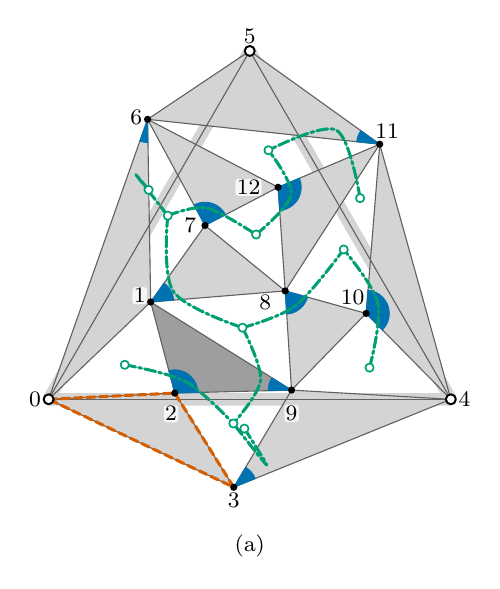
\begin{tikzpicture}[bf,x=0.04865\textwidth,y=0.04865\textwidth]
\draw[bfblack,line width=4.5pt,line join=round] (-4.330,-2.500)--(4.330,-2.500)--(0.000,5.000)--cycle;
\fill[bfblack] (-4.330,-2.500)--(-2.133,-0.405)--(-2.200,3.528)--cycle;
\fill[bfblack] (-4.330,-2.500)--(-1.614,-2.366)--(-0.344,-4.394)--cycle;
\fill[bfblack] (-2.133,-0.405)--(-0.963,1.243)--(0.764,-0.167)--cycle;
\fill[bfblack] (-2.133,-0.405)--(-1.614,-2.366)--(0.900,-2.302)--cycle;
\fill[bfblack] (-0.344,-4.394)--(4.330,-2.500)--(0.900,-2.302)--cycle;
\fill[bfblack] (4.330,-2.500)--(2.506,-0.651)--(2.799,2.992)--cycle;
\fill[bfblack] (0.000,5.000)--(-2.200,3.528)--(2.799,2.992)--cycle;
\fill[bfblack] (-2.200,3.528)--(-0.963,1.243)--(0.610,2.065)--cycle;
\fill[bfblack] (0.764,-0.167)--(2.799,2.992)--(0.610,2.065)--cycle;
\fill[bfblack] (0.764,-0.167)--(0.900,-2.302)--(2.506,-0.651)--cycle;
\fill[black!38] (-2.133,-0.405)--(-1.614,-2.366)--(0.900,-2.302)--cycle;
\draw[bf edge] (-4.330,-2.500)--(-2.133,-0.405);
\draw[bf edge] (-4.330,-2.500)--(-1.614,-2.366);
\draw[bf edge] (-4.330,-2.500)--(-0.344,-4.394);
\draw[bf edge] (-4.330,-2.500)--(4.330,-2.500);
\draw[bf edge] (-4.330,-2.500)--(0.000,5.000);
\draw[bf edge] (-4.330,-2.500)--(-2.200,3.528);
\draw[bf edge] (-2.133,-0.405)--(-1.614,-2.366);
\draw[bf edge] (-2.133,-0.405)--(-2.200,3.528);
\draw[bf edge] (-2.133,-0.405)--(-0.963,1.243);
\draw[bf edge] (-2.133,-0.405)--(0.764,-0.167);
\draw[bf edge] (-2.133,-0.405)--(0.900,-2.302);
\draw[bf edge] (-1.614,-2.366)--(-0.344,-4.394);
\draw[bf edge] (-1.614,-2.366)--(0.900,-2.302);
\draw[bf edge] (-0.344,-4.394)--(4.330,-2.500);
\draw[bf edge] (-0.344,-4.394)--(0.900,-2.302);
\draw[bf edge] (4.330,-2.500)--(0.000,5.000);
\draw[bf edge] (4.330,-2.500)--(0.900,-2.302);
\draw[bf edge] (4.330,-2.500)--(2.506,-0.651);
\draw[bf edge] (4.330,-2.500)--(2.799,2.992);
\draw[bf edge] (0.000,5.000)--(-2.200,3.528);
\draw[bf edge] (0.000,5.000)--(2.799,2.992);
\draw[bf edge] (-2.200,3.528)--(-0.963,1.243);
\draw[bf edge] (-2.200,3.528)--(2.799,2.992);
\draw[bf edge] (-2.200,3.528)--(0.610,2.065);
\draw[bf edge] (-0.963,1.243)--(0.764,-0.167);
\draw[bf edge] (-0.963,1.243)--(0.610,2.065);
\draw[bf edge] (0.764,-0.167)--(0.900,-2.302);
\draw[bf edge] (0.764,-0.167)--(2.506,-0.651);
\draw[bf edge] (0.764,-0.167)--(2.799,2.992);
\draw[bf edge] (0.764,-0.167)--(0.610,2.065);
\draw[bf edge] (0.900,-2.302)--(2.506,-0.651);
\draw[bf edge] (2.506,-0.651)--(2.799,2.992);
\draw[bf edge] (2.799,2.992)--(0.610,2.065);
\draw[bf Q] (-4.330,-2.500)--(-1.614,-2.366)--(-0.344,-4.394)--cycle;
\path[bf s] (-2.133,-0.405) -- ++(54.6:0.500) arc[start angle=54.6,end angle=4.7,radius=0.500] -- cycle;
\path[bf s] (-1.614,-2.366) -- ++(104.8:0.500) arc[start angle=104.8,end angle=1.5,radius=0.500] -- cycle;
\path[bf s] (-0.344,-4.394) -- ++(22.1:0.500) arc[start angle=22.1,end angle=59.3,radius=0.500] -- cycle;
\path[bf s] (-2.200,3.528) -- ++(-109.5:0.500) arc[start angle=-109.5,end angle=-89.0,radius=0.500] -- cycle;
\path[bf s] (-0.963,1.243) -- ++(118.4:0.500) arc[start angle=118.4,end angle=27.6,radius=0.500] -- cycle;
\path[bf s] (0.764,-0.167) -- ++(-86.4:0.500) arc[start angle=-86.4,end angle=-15.5,radius=0.500] -- cycle;
\path[bf s] (0.900,-2.302) -- ++(148.0:0.500) arc[start angle=148.0,end angle=181.5,radius=0.500] -- cycle;
\path[bf s] (2.506,-0.651) -- ++(-45.4:0.500) arc[start angle=-45.4,end angle=85.4,radius=0.500] -- cycle;
\path[bf s] (2.799,2.992) -- ++(144.3:0.500) arc[start angle=144.3,end angle=173.9,radius=0.500] -- cycle;
\path[bf s] (0.610,2.065) -- ++(-86.1:0.500) arc[start angle=-86.1,end angle=23.0,radius=0.500] -- cycle;
\draw[bf wtree] plot[smooth,tension=.55] coordinates {(-1.765,1.455) (-1.645,-0.179) (-0.156,-0.958)};
\draw[bf wtree] plot[smooth,tension=.55] coordinates {(-2.692,-1.757) (-1.375,-2.123) (-0.353,-3.021)};
\draw[bf wtree] plot[smooth,tension=.55] coordinates {(-0.115,-3.131) (0.366,-3.916) (-0.353,-3.021)};
\draw[bf wtree] plot[smooth,tension=.55] coordinates {(-2.177,2.009) (-2.448,2.333) (-1.765,1.455)};
\draw[bf wtree] plot[smooth,tension=.55] coordinates {(-1.765,1.455) (-0.923,1.616) (0.137,1.047)};
\draw[bf wtree] plot[smooth,tension=.55] coordinates {(-0.156,-0.958) (0.989,-0.481) (2.023,0.725)};
\draw[bf wtree] plot[smooth,tension=.55] coordinates {(-0.156,-0.958) (0.234,-2.082) (-0.353,-3.021)};
\draw[bf wtree] plot[smooth,tension=.55] coordinates {(2.579,-1.818) (2.760,-0.436) (2.023,0.725)};
\draw[bf wtree] plot[smooth,tension=.55] coordinates {(2.376,1.831) (1.863,3.297) (0.403,2.862)};
\draw[bf wtree] plot[smooth,tension=.55] coordinates {(0.137,1.047) (0.891,1.908) (0.403,2.862)};
\path[bf root] (-4.330,-2.500) circle[radius=1.8pt];
\path[bf vertex] (-2.133,-0.405) circle[radius=1.3pt];
\path[bf vertex] (-1.614,-2.366) circle[radius=1.3pt];
\path[bf vertex] (-0.344,-4.394) circle[radius=1.3pt];
\path[bf root] (4.330,-2.500) circle[radius=1.8pt];
\path[bf root] (0.000,5.000) circle[radius=1.8pt];
\path[bf vertex] (-2.200,3.528) circle[radius=1.3pt];
\path[bf vertex] (-0.963,1.243) circle[radius=1.3pt];
\path[bf vertex] (0.764,-0.167) circle[radius=1.3pt];
\path[bf vertex] (0.900,-2.302) circle[radius=1.3pt];
\path[bf vertex] (2.506,-0.651) circle[radius=1.3pt];
\path[bf vertex] (2.799,2.992) circle[radius=1.3pt];
\path[bf vertex] (0.610,2.065) circle[radius=1.3pt];
\path[draw=bfW,fill=white,line width=.6pt] (-2.692,-1.757) circle[radius=1.5pt];
\path[draw=bfW,fill=white,line width=.6pt] (-0.115,-3.131) circle[radius=1.5pt];
\path[draw=bfW,fill=white,line width=.6pt] (-2.177,2.009) circle[radius=1.5pt];
\path[draw=bfW,fill=white,line width=.6pt] (-1.765,1.455) circle[radius=1.5pt];
\path[draw=bfW,fill=white,line width=.6pt] (-0.156,-0.958) circle[radius=1.5pt];
\path[draw=bfW,fill=white,line width=.6pt] (-0.353,-3.021) circle[radius=1.5pt];
\path[draw=bfW,fill=white,line width=.6pt] (2.579,-1.818) circle[radius=1.5pt];
\path[draw=bfW,fill=white,line width=.6pt] (2.376,1.831) circle[radius=1.5pt];
\path[draw=bfW,fill=white,line width=.6pt] (0.403,2.862) circle[radius=1.5pt];
\path[draw=bfW,fill=white,line width=.6pt] (0.137,1.047) circle[radius=1.5pt];
\path[draw=bfW,fill=white,line width=.6pt] (2.023,0.725) circle[radius=1.5pt];
\node[fill=white,fill opacity=.8,text opacity=1,inner sep=.5pt,rounded corners=1pt] at (-4.625,-2.500) {$0$};
\node[fill=white,fill opacity=.8,text opacity=1,inner sep=.5pt,rounded corners=1pt] at (-2.369,-0.269) {$1$};
\node[fill=white,fill opacity=.8,text opacity=1,inner sep=.5pt,rounded corners=1pt] at (-1.693,-2.813) {$2$};
\node[fill=white,fill opacity=.8,text opacity=1,inner sep=.5pt,rounded corners=1pt] at (-0.344,-4.666) {$3$};
\node[fill=white,fill opacity=.8,text opacity=1,inner sep=.5pt,rounded corners=1pt] at (4.625,-2.500) {$4$};
\node[fill=white,fill opacity=.8,text opacity=1,inner sep=.5pt,rounded corners=1pt] at (0.000,5.318) {$5$};
\node[fill=white,fill opacity=.8,text opacity=1,inner sep=.5pt,rounded corners=1pt] at (-2.446,3.571) {$6$};
\node[fill=white,fill opacity=.8,text opacity=1,inner sep=.5pt,rounded corners=1pt] at (-1.281,1.243) {$7$};
\node[fill=white,fill opacity=.8,text opacity=1,inner sep=.5pt,rounded corners=1pt] at (0.332,-0.417) {$8$};
\node[fill=white,fill opacity=.8,text opacity=1,inner sep=.5pt,rounded corners=1pt] at (0.900,-2.801) {$9$};
\node[fill=white,fill opacity=.8,text opacity=1,inner sep=.5pt,rounded corners=1pt] at (2.214,-0.303) {$10$};
\node[fill=white,fill opacity=.8,text opacity=1,inner sep=.5pt,rounded corners=1pt] at (2.958,3.267) {$11$};
\node[fill=white,fill opacity=.8,text opacity=1,inner sep=.5pt,rounded corners=1pt] at (-0.025,2.065) {$12$};
\node[anchor=north] at (0.000,-5.344) {(a)};
\end{tikzpicture}%
\hspace{0.04\textwidth}%
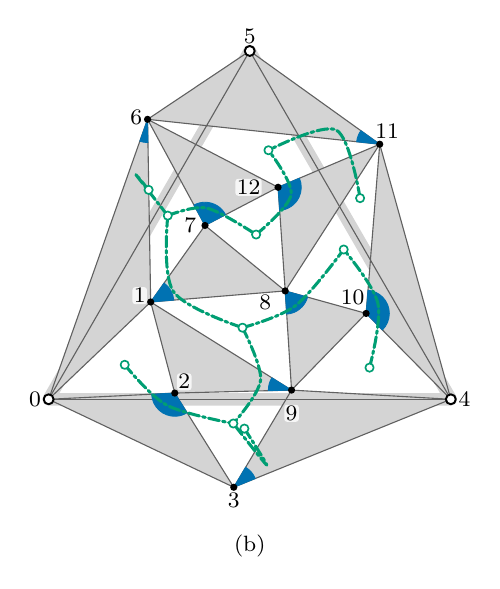
\begin{tikzpicture}[bf,x=0.04865\textwidth,y=0.04865\textwidth]
\draw[bfblack,line width=4.5pt,line join=round] (-4.330,-2.500)--(4.330,-2.500)--(0.000,5.000)--cycle;
\fill[bfblack] (-4.330,-2.500)--(-2.133,-0.405)--(-2.200,3.528)--cycle;
\fill[bfblack] (-4.330,-2.500)--(-1.614,-2.366)--(-0.344,-4.394)--cycle;
\fill[bfblack] (-2.133,-0.405)--(-0.963,1.243)--(0.764,-0.167)--cycle;
\fill[bfblack] (-2.133,-0.405)--(-1.614,-2.366)--(0.900,-2.302)--cycle;
\fill[bfblack] (-0.344,-4.394)--(4.330,-2.500)--(0.900,-2.302)--cycle;
\fill[bfblack] (4.330,-2.500)--(2.506,-0.651)--(2.799,2.992)--cycle;
\fill[bfblack] (0.000,5.000)--(-2.200,3.528)--(2.799,2.992)--cycle;
\fill[bfblack] (-2.200,3.528)--(-0.963,1.243)--(0.610,2.065)--cycle;
\fill[bfblack] (0.764,-0.167)--(2.799,2.992)--(0.610,2.065)--cycle;
\fill[bfblack] (0.764,-0.167)--(0.900,-2.302)--(2.506,-0.651)--cycle;
\draw[bf edge] (-4.330,-2.500)--(-2.133,-0.405);
\draw[bf edge] (-4.330,-2.500)--(-1.614,-2.366);
\draw[bf edge] (-4.330,-2.500)--(-0.344,-4.394);
\draw[bf edge] (-4.330,-2.500)--(4.330,-2.500);
\draw[bf edge] (-4.330,-2.500)--(0.000,5.000);
\draw[bf edge] (-4.330,-2.500)--(-2.200,3.528);
\draw[bf edge] (-2.133,-0.405)--(-1.614,-2.366);
\draw[bf edge] (-2.133,-0.405)--(-2.200,3.528);
\draw[bf edge] (-2.133,-0.405)--(-0.963,1.243);
\draw[bf edge] (-2.133,-0.405)--(0.764,-0.167);
\draw[bf edge] (-2.133,-0.405)--(0.900,-2.302);
\draw[bf edge] (-1.614,-2.366)--(-0.344,-4.394);
\draw[bf edge] (-1.614,-2.366)--(0.900,-2.302);
\draw[bf edge] (-0.344,-4.394)--(4.330,-2.500);
\draw[bf edge] (-0.344,-4.394)--(0.900,-2.302);
\draw[bf edge] (4.330,-2.500)--(0.000,5.000);
\draw[bf edge] (4.330,-2.500)--(0.900,-2.302);
\draw[bf edge] (4.330,-2.500)--(2.506,-0.651);
\draw[bf edge] (4.330,-2.500)--(2.799,2.992);
\draw[bf edge] (0.000,5.000)--(-2.200,3.528);
\draw[bf edge] (0.000,5.000)--(2.799,2.992);
\draw[bf edge] (-2.200,3.528)--(-0.963,1.243);
\draw[bf edge] (-2.200,3.528)--(2.799,2.992);
\draw[bf edge] (-2.200,3.528)--(0.610,2.065);
\draw[bf edge] (-0.963,1.243)--(0.764,-0.167);
\draw[bf edge] (-0.963,1.243)--(0.610,2.065);
\draw[bf edge] (0.764,-0.167)--(0.900,-2.302);
\draw[bf edge] (0.764,-0.167)--(2.506,-0.651);
\draw[bf edge] (0.764,-0.167)--(2.799,2.992);
\draw[bf edge] (0.764,-0.167)--(0.610,2.065);
\draw[bf edge] (0.900,-2.302)--(2.506,-0.651);
\draw[bf edge] (2.506,-0.651)--(2.799,2.992);
\draw[bf edge] (2.799,2.992)--(0.610,2.065);
\path[bf s] (-2.133,-0.405) -- ++(54.6:0.500) arc[start angle=54.6,end angle=4.7,radius=0.500] -- cycle;
\path[bf s] (-1.614,-2.366) -- ++(-177.2:0.500) arc[start angle=-177.2,end angle=-57.9,radius=0.500] -- cycle;
\path[bf s] (-0.344,-4.394) -- ++(22.1:0.500) arc[start angle=22.1,end angle=59.3,radius=0.500] -- cycle;
\path[bf s] (-2.200,3.528) -- ++(-109.5:0.500) arc[start angle=-109.5,end angle=-89.0,radius=0.500] -- cycle;
\path[bf s] (-0.963,1.243) -- ++(118.4:0.500) arc[start angle=118.4,end angle=27.6,radius=0.500] -- cycle;
\path[bf s] (0.764,-0.167) -- ++(-86.4:0.500) arc[start angle=-86.4,end angle=-15.5,radius=0.500] -- cycle;
\path[bf s] (0.900,-2.302) -- ++(148.0:0.500) arc[start angle=148.0,end angle=181.5,radius=0.500] -- cycle;
\path[bf s] (2.506,-0.651) -- ++(-45.4:0.500) arc[start angle=-45.4,end angle=85.4,radius=0.500] -- cycle;
\path[bf s] (2.799,2.992) -- ++(144.3:0.500) arc[start angle=144.3,end angle=173.9,radius=0.500] -- cycle;
\path[bf s] (0.610,2.065) -- ++(-86.1:0.500) arc[start angle=-86.1,end angle=23.0,radius=0.500] -- cycle;
\draw[bf wtree] plot[smooth,tension=.55] coordinates {(-1.765,1.455) (-1.645,-0.179) (-0.156,-0.958)};
\draw[bf wtree] plot[smooth,tension=.55] coordinates {(-2.692,-1.757) (-1.788,-2.625) (-0.353,-3.021)};
\draw[bf wtree] plot[smooth,tension=.55] coordinates {(-0.115,-3.131) (0.366,-3.916) (-0.353,-3.021)};
\draw[bf wtree] plot[smooth,tension=.55] coordinates {(-2.177,2.009) (-2.448,2.333) (-1.765,1.455)};
\draw[bf wtree] plot[smooth,tension=.55] coordinates {(-1.765,1.455) (-0.923,1.616) (0.137,1.047)};
\draw[bf wtree] plot[smooth,tension=.55] coordinates {(-0.156,-0.958) (0.989,-0.481) (2.023,0.725)};
\draw[bf wtree] plot[smooth,tension=.55] coordinates {(-0.156,-0.958) (0.234,-2.082) (-0.353,-3.021)};
\draw[bf wtree] plot[smooth,tension=.55] coordinates {(2.579,-1.818) (2.760,-0.436) (2.023,0.725)};
\draw[bf wtree] plot[smooth,tension=.55] coordinates {(2.376,1.831) (1.863,3.297) (0.403,2.862)};
\draw[bf wtree] plot[smooth,tension=.55] coordinates {(0.137,1.047) (0.891,1.908) (0.403,2.862)};
\path[bf root] (-4.330,-2.500) circle[radius=1.8pt];
\path[bf vertex] (-2.133,-0.405) circle[radius=1.3pt];
\path[bf vertex] (-1.614,-2.366) circle[radius=1.3pt];
\path[bf vertex] (-0.344,-4.394) circle[radius=1.3pt];
\path[bf root] (4.330,-2.500) circle[radius=1.8pt];
\path[bf root] (0.000,5.000) circle[radius=1.8pt];
\path[bf vertex] (-2.200,3.528) circle[radius=1.3pt];
\path[bf vertex] (-0.963,1.243) circle[radius=1.3pt];
\path[bf vertex] (0.764,-0.167) circle[radius=1.3pt];
\path[bf vertex] (0.900,-2.302) circle[radius=1.3pt];
\path[bf vertex] (2.506,-0.651) circle[radius=1.3pt];
\path[bf vertex] (2.799,2.992) circle[radius=1.3pt];
\path[bf vertex] (0.610,2.065) circle[radius=1.3pt];
\path[draw=bfW,fill=white,line width=.6pt] (-2.692,-1.757) circle[radius=1.5pt];
\path[draw=bfW,fill=white,line width=.6pt] (-0.115,-3.131) circle[radius=1.5pt];
\path[draw=bfW,fill=white,line width=.6pt] (-2.177,2.009) circle[radius=1.5pt];
\path[draw=bfW,fill=white,line width=.6pt] (-1.765,1.455) circle[radius=1.5pt];
\path[draw=bfW,fill=white,line width=.6pt] (-0.156,-0.958) circle[radius=1.5pt];
\path[draw=bfW,fill=white,line width=.6pt] (-0.353,-3.021) circle[radius=1.5pt];
\path[draw=bfW,fill=white,line width=.6pt] (2.579,-1.818) circle[radius=1.5pt];
\path[draw=bfW,fill=white,line width=.6pt] (2.376,1.831) circle[radius=1.5pt];
\path[draw=bfW,fill=white,line width=.6pt] (0.403,2.862) circle[radius=1.5pt];
\path[draw=bfW,fill=white,line width=.6pt] (0.137,1.047) circle[radius=1.5pt];
\path[draw=bfW,fill=white,line width=.6pt] (2.023,0.725) circle[radius=1.5pt];
\node[fill=white,fill opacity=.8,text opacity=1,inner sep=.5pt,rounded corners=1pt] at (-4.625,-2.500) {$0$};
\node[fill=white,fill opacity=.8,text opacity=1,inner sep=.5pt,rounded corners=1pt] at (-2.369,-0.269) {$1$};
\node[fill=white,fill opacity=.8,text opacity=1,inner sep=.5pt,rounded corners=1pt] at (-1.410,-2.123) {$2$};
\node[fill=white,fill opacity=.8,text opacity=1,inner sep=.5pt,rounded corners=1pt] at (-0.344,-4.666) {$3$};
\node[fill=white,fill opacity=.8,text opacity=1,inner sep=.5pt,rounded corners=1pt] at (4.625,-2.500) {$4$};
\node[fill=white,fill opacity=.8,text opacity=1,inner sep=.5pt,rounded corners=1pt] at (0.000,5.318) {$5$};
\node[fill=white,fill opacity=.8,text opacity=1,inner sep=.5pt,rounded corners=1pt] at (-2.446,3.571) {$6$};
\node[fill=white,fill opacity=.8,text opacity=1,inner sep=.5pt,rounded corners=1pt] at (-1.281,1.243) {$7$};
\node[fill=white,fill opacity=.8,text opacity=1,inner sep=.5pt,rounded corners=1pt] at (0.332,-0.417) {$8$};
\node[fill=white,fill opacity=.8,text opacity=1,inner sep=.5pt,rounded corners=1pt] at (0.900,-2.801) {$9$};
\node[fill=white,fill opacity=.8,text opacity=1,inner sep=.5pt,rounded corners=1pt] at (2.214,-0.303) {$10$};
\node[fill=white,fill opacity=.8,text opacity=1,inner sep=.5pt,rounded corners=1pt] at (2.958,3.267) {$11$};
\node[fill=white,fill opacity=.8,text opacity=1,inner sep=.5pt,rounded corners=1pt] at (-0.025,2.065) {$12$};
\node[anchor=north] at (0.000,-5.344) {(b)};
\end{tikzpicture}%
\end{minipage}}
\caption{Two rainbow trees in the example of \cite[Figure~2]{Paper}, with $13$ vertices and roots $0,4,5$. Black faces are shaded and the grey ring stands for $t_0$. A wedge in the face $\sigma(x)$ at $x$ marks each removed arc $x\sigma(x)$, and the dash-dotted edges $(x\sigma(x))^*$ form a spanning tree of $W$, whose $11$ vertices are drawn as small circles. (a) Excess $2$: the dark face $\{1,2,9\}$ has load $2$ and the face $\{0,2,3\}$ with the dashed outline has load $0$. (b) Excess $0$, a good state. The example has $1792$ rainbow trees, six of them good states.}
\label{fig:rainbow}
\end{figure}

\section{When a rainbow tree exists}\label{sec:R}

Let $\Delta$ be a separating triangle of $T$.
Its \emph{inner side} is the side that does not contain $t_0$, and $\Delta$ has \emph{three black faces along its inner side} if the three faces of $T$ at the edges of $\Delta$ that lie on this side are black.
We use Rado's theorem in the following form \cite{Rado}, \cite[Exercise~10.26]{SchrijverCourse}: subsets $E_1,\dots,E_k$ of the ground set of a matroid have an independent transversal if and only if the union of any $j$ of them has rank at least $j$.

\begin{theorem}\label{thm:R}
$T$ has a rainbow tree if and only if no separating triangle of $T$ has three black faces along its inner side.
\end{theorem}

\begin{proof}
For $x\in X$ let $E_x$ be the set of the edges $(xt)^*$ of $W$, over the black faces $t$ at $x$.
These sets are disjoint, and $E_x$ is the edge set of a closed walk through the white faces at $x$.
By Lemma~\ref{lem:dual} a rainbow tree is an independent transversal of $(E_x)_{x\in X}$ in the cycle matroid of $W$, whose rank is $n$.
Two walks $E_x$ and $E_{x'}$ share a white face exactly when $xx'$ is an edge of $T$.
So for $J\subseteq X$ the union of the $E_x$, $x\in J$, has one component for each component of the induced subgraph $T[J]$, and different components use disjoint sets of white faces.
Its rank is the number $w(J)$ of white faces with a corner in $J$, minus the number of components of $T[J]$.
Both $w(J)$ and $|J|$ add over the components of $T[J]$, so by Rado's theorem a rainbow tree exists if and only if
\begin{equation}\label{eq:rado}
w(J)\ \ge\ |J|+1\qquad\text{for every nonempty } J\subseteq X \text{ with } T[J] \text{ connected.}
\end{equation}

Fix such a $J$.
Let $U=V(T)\setminus J$, which contains the roots, and let $T[U]$ have $p$ vertices, $q$ edges and $\kappa$ components.
The connected set $J$ lies in one face $\Phi$ of the plane graph $T[U]$.
Every other face of $T[U]$ contains no vertex of $T$ and no edge of $T$, since such an edge would join two vertices of $U$ and belong to $T[U]$; so it is a face of $T$.
Conversely a face of $T$ with all corners in $U$ is a face of $T[U]$ other than $\Phi$.
Let $b_U$ and $w_U$ be the numbers of black and of white faces of $T$ with all corners in $U$.
Let $d$ be the number of edge sides on the boundary of $\Phi$, and $\varsigma$ the sum over these sides of $+1$ or $-1$ according as the face of $T$ in $\Phi$ at this side is black or white.
Then
\[
p-q+(b_U+w_U+1)=1+\kappa,\qquad 2q=3(b_U+w_U)+d,\qquad \varsigma=3(w_U-b_U).
\]
The first is Euler's formula and the second counts edge sides.
For the third, give every black face of $T$ in $\Phi$ the value $+1$ and every white one the value $-1$ on each of its three sides.
There are $n+1-b_U$ black and $n+1-w_U$ white faces in $\Phi$, the two sides of an edge inside $\Phi$ cancel, and the boundary sides remain.
Solving, $w_U=p-\kappa-d/2+\varsigma/6$.
Since $w(J)=n+1-w_U$ and $|J|=n+3-p$,
\begin{equation}\label{eq:euler}
w(J)-|J|-1\ =\ (\kappa-1)+\frac{3d-\varsigma-12}{6}.
\end{equation}

The number $\varsigma$ is a multiple of $3$ with the parity of $d$, and $|\varsigma|\le d$.
The component of $T[U]$ that contains the roots has a vertex adjacent to $J$, so it borders $\Phi$, and it is not a tree, so $d\ge3$.
If $\kappa\ge2$, the right side of \eqref{eq:euler} is at least $1+(2d-12)/6=(d-3)/3\ge0$.
Let $\kappa=1$.
If $d=4$ then $\varsigma=0$, if $d=5$ then $\varsigma\le3$, and if $d\ge6$ then $3d-\varsigma\ge2d\ge12$; in each case the right side is at least $0$.
If $d=3$, the right side is negative only for $\varsigma=3$.
The boundary of $\Phi$ is then a triangle $\Delta$, the three faces along it in $\Phi$ are black, and $t_0$ lies on the other side.
If the other side contained no vertex, it would be the face $t_0$, and the faces along $\Delta$ in $\Phi$ would be white.
So $\Delta$ is a separating triangle with three black faces along its inner side.
This proves \eqref{eq:rado} when there is no such triangle.

Conversely let $\Delta$ be a separating triangle with three black faces along its inner side, and let $J$ be the set of the $I\ge1$ vertices on this side.
Let $b_\Delta$ and $w_\Delta$ be the numbers of black and of white faces on the inner side.
Euler's formula and the count of sides for the disk give $b_\Delta+w_\Delta=2I+1$, and the signed count of sides gives $3(b_\Delta-w_\Delta)=3$.
So $w_\Delta=I$ and $b_\Delta=I+1$.
Every white face with a corner in $J$ lies on the inner side, so $w(J)\le|J|$ and the union of the $E_x$, $x\in J$, has rank less than $|J|$.
By Rado's theorem there is no rainbow tree.
\end{proof}

Rado's theorem is a case of matroid intersection, so a rainbow tree can be found in polynomial time when one exists.

\section{Each rainbow tree lies in one \texorpdfstring{$2$}{2}-factor}\label{sec:S}

Let $F$ be a $2$-factor of $H$.
A map $\sigma\colon X\to A$ \emph{lies in} $F$ if $x\sigma(x)$ is an edge of $F$ for every $x\in X$, and a state lies in $F$ if its inverse does.
For $t\in A$ let $u(t)$ be the corner of $t$ that is not joined to $t$ in $F$; for a pair $(r,s)$ with $2$-factor $F$ this is the third corner $u(t)$ of \cite[Section~4]{Paper}.
Let $D_F$ be the directed graph on $V(T)$ with an arc $v\to u(t)$ for each of the two corners $v$ of $t$ joined to $t$ in $F$, for every $t\in A$.
Its arcs run along the two sides of $t$ at $u(t)$.
Every vertex of $X$ has outdegree two in $D_F$, one arc through each of its two faces in $F$, and the roots have outdegree zero (Figure~\ref{fig:digraph}).
For a pair $(r,s)$ with $2$-factor $F$, the arcs of $D_F$ are the edges of $Q_s$, directed by $r$ from $r(t)$ to $u(t)$, and the edges of $Q_r$, directed by $s$ from $s(t)$ to $u(t)$.

\begin{lemma}\label{lem:orient}
Let $F$ be a $2$-factor of $H$, let $\sigma\colon X\to A$ lie in $F$, and for $x\in X$ let $x\sigma'(x)$ be the other edge of $F$ at $x$.
Then $H_\sigma$ is a spanning tree of $\Hp$ if and only if the $n$ arcs $x\to u(\sigma'(x))$ of $D_F$ contain no directed cycle.
In that case $p_{\sigma'(x)}$ is the parent of $x$ in $H_\sigma$ rooted at $p_{t_0}$.
\end{lemma}

\begin{proof}
Direct the arc $x\sigma'(x)$ from $x$ to $p_{\sigma'(x)}$, the arc $u(t)t$ from $p_t$ to $u(t)$ for $t\in A$, and the three arcs at $p_{t_0}$ from the roots to $p_{t_0}$.
An arc $vt$ with $t\in A$ that is not an edge of $F$ has $v=u(t)$, so these are all $2n+3$ arcs of $H_\sigma$ and each has one direction.
Every vertex of $\Hp$ except $p_{t_0}$ has outdegree one.
A graph with $|V(\Hp)|-1$ edges directed in this way is a spanning tree if and only if it has no directed cycle, and its edges then point to the parents.
A directed cycle avoids the roots, so it alternates $x\to p_{\sigma'(x)}\to u(\sigma'(x))$.
\end{proof}

For a rainbow tree $\sigma$ and $x\in X$, let $\parent_\sigma(x)$ be the black face $t$ such that $p_t$ is the parent of $x$ in $H_\sigma$ rooted at $p_{t_0}$.

\begin{theorem}\label{thm:S}
\begin{enumerate}
\item Every rainbow tree $\sigma$ lies in exactly one $2$-factor of $H$, namely the one with the edges $x\sigma(x)$ and $x\parent_\sigma(x)$, $x\in X$.
\item Let $F$ be a $2$-factor of $H$. The rainbow trees in $F$ correspond to the sets of arcs of $D_F$ that contain one arc out of every vertex of $X$ and no directed cycle; $\sigma$ corresponds to the arcs $x\to u(\sigma'(x))$. Such a set is a spanning forest of $D_F$ directed towards the roots. The good states in $F$ correspond to the sets that contain exactly one of the two arcs of every face.
\item $D_F$ has a directed cycle if and only if $H$ has a $2$-factor other than $F$. If $F$ is the only $2$-factor of $H$, then all $2^n$ maps $\sigma$ that lie in $F$ are rainbow trees and all states in $F$ are good.
\end{enumerate}
\end{theorem}

\begin{proof}
(1) In $H_\sigma$ the neighbours of $x\in X$ are the points of the black faces at $x$ other than $\sigma(x)$, all of them in $A$.
So $\parent_\sigma(x)\in A$ and $\parent_\sigma(x)\ne\sigma(x)$.
The point $p_t$ of $t\in A$ has $3-\lambda_\sigma(t)$ neighbours, one of them its parent, so $t$ is $\parent_\sigma(x)$ for $2-\lambda_\sigma(t)$ vertices $x$, none of them a root.
Hence every $t$ lies on $\lambda_\sigma(t)+2-\lambda_\sigma(t)=2$ of the edges $x\sigma(x)$ and $x\parent_\sigma(x)$, which therefore form a $2$-factor.
If $\sigma$ lies in a $2$-factor $F$, then $\sigma'=\parent_\sigma$ by Lemma~\ref{lem:orient}.

(2) The first sentence is Lemma~\ref{lem:orient}. A set of $n$ arcs with one arc out of every vertex of $X$ and no directed cycle leads from every vertex to a root. The arc from $v$ through $t$ is chosen exactly when $\sigma'(v)=t$, so one arc in every face means that $\sigma'$ is a bijection, and then so is $\sigma$.

(3) Let $v_1\to v_2\to\dots\to v_k\to v_1$ be a directed cycle of $D_F$, the arc $v_i\to v_{i+1}$ running through $t_i$.
Then $u(t_i)=v_{i+1}$, so the $t_i$ are distinct, and replacing every edge $v_it_i$ of $F$ by $v_{i+1}t_i$ gives another $2$-factor.
Conversely let $F'\ne F$ be a $2$-factor of $H$.
Every vertex of $H$ meets as many edges of $F\setminus F'$ as of $F'\setminus F$, so the symmetric difference splits into closed trails that alternate between the two.
An edge $vt$ of $F'\setminus F$ has $v=u(t)$, so each trail is a closed directed walk in $D_F$, which contains a directed cycle.
The last sentence follows from (2).
\end{proof}

\begin{figure}[H]
\centering
\scalebox{.9}{\begin{minipage}{\textwidth}\centering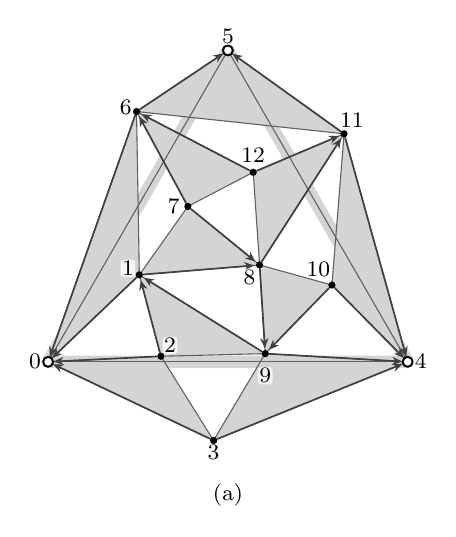
\begin{tikzpicture}[bf,x=0.04348\textwidth,y=0.04348\textwidth]
\draw[bfblack,line width=4.5pt,line join=round] (-4.330,-2.500)--(4.330,-2.500)--(0.000,5.000)--cycle;
\fill[bfblack] (-4.330,-2.500)--(-2.133,-0.405)--(-2.200,3.528)--cycle;
\fill[bfblack] (-4.330,-2.500)--(-1.614,-2.366)--(-0.344,-4.394)--cycle;
\fill[bfblack] (-2.133,-0.405)--(-0.963,1.243)--(0.764,-0.167)--cycle;
\fill[bfblack] (-2.133,-0.405)--(-1.614,-2.366)--(0.900,-2.302)--cycle;
\fill[bfblack] (-0.344,-4.394)--(4.330,-2.500)--(0.900,-2.302)--cycle;
\fill[bfblack] (4.330,-2.500)--(2.506,-0.651)--(2.799,2.992)--cycle;
\fill[bfblack] (0.000,5.000)--(-2.200,3.528)--(2.799,2.992)--cycle;
\fill[bfblack] (-2.200,3.528)--(-0.963,1.243)--(0.610,2.065)--cycle;
\fill[bfblack] (0.764,-0.167)--(2.799,2.992)--(0.610,2.065)--cycle;
\fill[bfblack] (0.764,-0.167)--(0.900,-2.302)--(2.506,-0.651)--cycle;
\draw[bf edge] (-4.330,-2.500)--(-2.133,-0.405);
\draw[bf edge] (-4.330,-2.500)--(-1.614,-2.366);
\draw[bf edge] (-4.330,-2.500)--(-0.344,-4.394);
\draw[bf edge] (-4.330,-2.500)--(4.330,-2.500);
\draw[bf edge] (-4.330,-2.500)--(0.000,5.000);
\draw[bf edge] (-4.330,-2.500)--(-2.200,3.528);
\draw[bf edge] (-2.133,-0.405)--(-1.614,-2.366);
\draw[bf edge] (-2.133,-0.405)--(-2.200,3.528);
\draw[bf edge] (-2.133,-0.405)--(-0.963,1.243);
\draw[bf edge] (-2.133,-0.405)--(0.764,-0.167);
\draw[bf edge] (-2.133,-0.405)--(0.900,-2.302);
\draw[bf edge] (-1.614,-2.366)--(-0.344,-4.394);
\draw[bf edge] (-1.614,-2.366)--(0.900,-2.302);
\draw[bf edge] (-0.344,-4.394)--(4.330,-2.500);
\draw[bf edge] (-0.344,-4.394)--(0.900,-2.302);
\draw[bf edge] (4.330,-2.500)--(0.000,5.000);
\draw[bf edge] (4.330,-2.500)--(0.900,-2.302);
\draw[bf edge] (4.330,-2.500)--(2.506,-0.651);
\draw[bf edge] (4.330,-2.500)--(2.799,2.992);
\draw[bf edge] (0.000,5.000)--(-2.200,3.528);
\draw[bf edge] (0.000,5.000)--(2.799,2.992);
\draw[bf edge] (-2.200,3.528)--(-0.963,1.243);
\draw[bf edge] (-2.200,3.528)--(2.799,2.992);
\draw[bf edge] (-2.200,3.528)--(0.610,2.065);
\draw[bf edge] (-0.963,1.243)--(0.764,-0.167);
\draw[bf edge] (-0.963,1.243)--(0.610,2.065);
\draw[bf edge] (0.764,-0.167)--(0.900,-2.302);
\draw[bf edge] (0.764,-0.167)--(2.506,-0.651);
\draw[bf edge] (0.764,-0.167)--(2.799,2.992);
\draw[bf edge] (0.764,-0.167)--(0.610,2.065);
\draw[bf edge] (0.900,-2.302)--(2.506,-0.651);
\draw[bf edge] (2.506,-0.651)--(2.799,2.992);
\draw[bf edge] (2.799,2.992)--(0.610,2.065);
\draw[bf arc] (-2.133,-0.405) to[bend left=0] (-4.330,-2.500);
\draw[bf arc] (-2.200,3.528) to[bend left=0] (-4.330,-2.500);
\draw[bf arc] (-1.614,-2.366) to[bend left=0] (-4.330,-2.500);
\draw[bf arc] (-0.344,-4.394) to[bend left=0] (-4.330,-2.500);
\draw[bf arc] (-2.133,-0.405) to[bend left=0] (0.764,-0.167);
\draw[bf arc] (-0.963,1.243) to[bend left=0] (0.764,-0.167);
\draw[bf arc] (-1.614,-2.366) to[bend left=0] (-2.133,-0.405);
\draw[bf arc] (0.900,-2.302) to[bend left=0] (-2.133,-0.405);
\draw[bf arc] (-0.344,-4.394) to[bend left=0] (4.330,-2.500);
\draw[bf arc] (0.900,-2.302) to[bend left=0] (4.330,-2.500);
\draw[bf arc] (2.506,-0.651) to[bend left=0] (4.330,-2.500);
\draw[bf arc] (2.799,2.992) to[bend left=0] (4.330,-2.500);
\draw[bf arc] (-2.200,3.528) to[bend left=0] (0.000,5.000);
\draw[bf arc] (2.799,2.992) to[bend left=0] (0.000,5.000);
\draw[bf arc] (-0.963,1.243) to[bend left=0] (-2.200,3.528);
\draw[bf arc] (0.610,2.065) to[bend left=0] (-2.200,3.528);
\draw[bf arc] (0.764,-0.167) to[bend left=0] (2.799,2.992);
\draw[bf arc] (0.610,2.065) to[bend left=0] (2.799,2.992);
\draw[bf arc] (0.764,-0.167) to[bend left=0] (0.900,-2.302);
\draw[bf arc] (2.506,-0.651) to[bend left=0] (0.900,-2.302);
\path[bf root] (-4.330,-2.500) circle[radius=1.8pt];
\path[bf vertex] (-2.133,-0.405) circle[radius=1.3pt];
\path[bf vertex] (-1.614,-2.366) circle[radius=1.3pt];
\path[bf vertex] (-0.344,-4.394) circle[radius=1.3pt];
\path[bf root] (4.330,-2.500) circle[radius=1.8pt];
\path[bf root] (0.000,5.000) circle[radius=1.8pt];
\path[bf vertex] (-2.200,3.528) circle[radius=1.3pt];
\path[bf vertex] (-0.963,1.243) circle[radius=1.3pt];
\path[bf vertex] (0.764,-0.167) circle[radius=1.3pt];
\path[bf vertex] (0.900,-2.302) circle[radius=1.3pt];
\path[bf vertex] (2.506,-0.651) circle[radius=1.3pt];
\path[bf vertex] (2.799,2.992) circle[radius=1.3pt];
\path[bf vertex] (0.610,2.065) circle[radius=1.3pt];
\node[fill=white,fill opacity=.8,text opacity=1,inner sep=.5pt,rounded corners=1pt] at (-4.647,-2.500) {$0$};
\node[fill=white,fill opacity=.8,text opacity=1,inner sep=.5pt,rounded corners=1pt] at (-2.408,-0.246) {$1$};
\node[fill=white,fill opacity=.8,text opacity=1,inner sep=.5pt,rounded corners=1pt] at (-1.394,-2.103) {$2$};
\node[fill=white,fill opacity=.8,text opacity=1,inner sep=.5pt,rounded corners=1pt] at (-0.344,-4.686) {$3$};
\node[fill=white,fill opacity=.8,text opacity=1,inner sep=.5pt,rounded corners=1pt] at (4.647,-2.500) {$4$};
\node[fill=white,fill opacity=.8,text opacity=1,inner sep=.5pt,rounded corners=1pt] at (0.000,5.343) {$5$};
\node[fill=white,fill opacity=.8,text opacity=1,inner sep=.5pt,rounded corners=1pt] at (-2.462,3.624) {$6$};
\node[fill=white,fill opacity=.8,text opacity=1,inner sep=.5pt,rounded corners=1pt] at (-1.306,1.243) {$7$};
\node[fill=white,fill opacity=.8,text opacity=1,inner sep=.5pt,rounded corners=1pt] at (0.519,-0.459) {$8$};
\node[fill=white,fill opacity=.8,text opacity=1,inner sep=.5pt,rounded corners=1pt] at (0.900,-2.835) {$9$};
\node[fill=white,fill opacity=.8,text opacity=1,inner sep=.5pt,rounded corners=1pt] at (2.180,-0.262) {$10$};
\node[fill=white,fill opacity=.8,text opacity=1,inner sep=.5pt,rounded corners=1pt] at (2.989,3.322) {$11$};
\node[fill=white,fill opacity=.8,text opacity=1,inner sep=.5pt,rounded corners=1pt] at (0.610,2.471) {$12$};
\node[anchor=north] at (0.000,-5.344) {(a)};
\end{tikzpicture}%
\hspace{0.04\textwidth}%
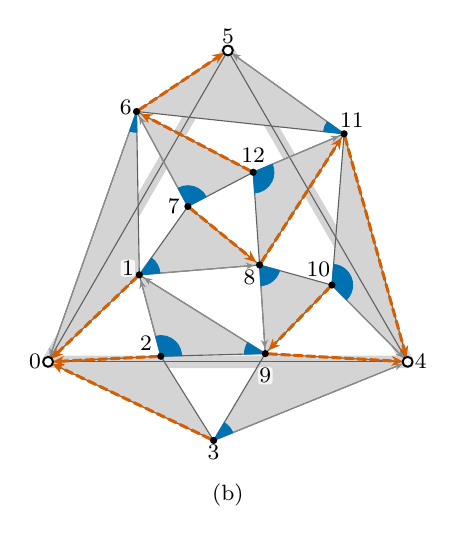
\begin{tikzpicture}[bf,x=0.04348\textwidth,y=0.04348\textwidth]
\draw[bfblack,line width=4.5pt,line join=round] (-4.330,-2.500)--(4.330,-2.500)--(0.000,5.000)--cycle;
\fill[bfblack] (-4.330,-2.500)--(-2.133,-0.405)--(-2.200,3.528)--cycle;
\fill[bfblack] (-4.330,-2.500)--(-1.614,-2.366)--(-0.344,-4.394)--cycle;
\fill[bfblack] (-2.133,-0.405)--(-0.963,1.243)--(0.764,-0.167)--cycle;
\fill[bfblack] (-2.133,-0.405)--(-1.614,-2.366)--(0.900,-2.302)--cycle;
\fill[bfblack] (-0.344,-4.394)--(4.330,-2.500)--(0.900,-2.302)--cycle;
\fill[bfblack] (4.330,-2.500)--(2.506,-0.651)--(2.799,2.992)--cycle;
\fill[bfblack] (0.000,5.000)--(-2.200,3.528)--(2.799,2.992)--cycle;
\fill[bfblack] (-2.200,3.528)--(-0.963,1.243)--(0.610,2.065)--cycle;
\fill[bfblack] (0.764,-0.167)--(2.799,2.992)--(0.610,2.065)--cycle;
\fill[bfblack] (0.764,-0.167)--(0.900,-2.302)--(2.506,-0.651)--cycle;
\draw[bf edge] (-4.330,-2.500)--(-2.133,-0.405);
\draw[bf edge] (-4.330,-2.500)--(-1.614,-2.366);
\draw[bf edge] (-4.330,-2.500)--(-0.344,-4.394);
\draw[bf edge] (-4.330,-2.500)--(4.330,-2.500);
\draw[bf edge] (-4.330,-2.500)--(0.000,5.000);
\draw[bf edge] (-4.330,-2.500)--(-2.200,3.528);
\draw[bf edge] (-2.133,-0.405)--(-1.614,-2.366);
\draw[bf edge] (-2.133,-0.405)--(-2.200,3.528);
\draw[bf edge] (-2.133,-0.405)--(-0.963,1.243);
\draw[bf edge] (-2.133,-0.405)--(0.764,-0.167);
\draw[bf edge] (-2.133,-0.405)--(0.900,-2.302);
\draw[bf edge] (-1.614,-2.366)--(-0.344,-4.394);
\draw[bf edge] (-1.614,-2.366)--(0.900,-2.302);
\draw[bf edge] (-0.344,-4.394)--(4.330,-2.500);
\draw[bf edge] (-0.344,-4.394)--(0.900,-2.302);
\draw[bf edge] (4.330,-2.500)--(0.000,5.000);
\draw[bf edge] (4.330,-2.500)--(0.900,-2.302);
\draw[bf edge] (4.330,-2.500)--(2.506,-0.651);
\draw[bf edge] (4.330,-2.500)--(2.799,2.992);
\draw[bf edge] (0.000,5.000)--(-2.200,3.528);
\draw[bf edge] (0.000,5.000)--(2.799,2.992);
\draw[bf edge] (-2.200,3.528)--(-0.963,1.243);
\draw[bf edge] (-2.200,3.528)--(2.799,2.992);
\draw[bf edge] (-2.200,3.528)--(0.610,2.065);
\draw[bf edge] (-0.963,1.243)--(0.764,-0.167);
\draw[bf edge] (-0.963,1.243)--(0.610,2.065);
\draw[bf edge] (0.764,-0.167)--(0.900,-2.302);
\draw[bf edge] (0.764,-0.167)--(2.506,-0.651);
\draw[bf edge] (0.764,-0.167)--(2.799,2.992);
\draw[bf edge] (0.764,-0.167)--(0.610,2.065);
\draw[bf edge] (0.900,-2.302)--(2.506,-0.651);
\draw[bf edge] (2.506,-0.651)--(2.799,2.992);
\draw[bf edge] (2.799,2.992)--(0.610,2.065);
\draw[bf Qdir] (-2.133,-0.405) to[bend left=0] (-4.330,-2.500);
\draw[bf arc faint] (-2.200,3.528) to[bend left=0] (-4.330,-2.500);
\draw[bf Qdir] (-1.614,-2.366) to[bend left=0] (-4.330,-2.500);
\draw[bf Qdir] (-0.344,-4.394) to[bend left=0] (-4.330,-2.500);
\draw[bf arc faint] (-2.133,-0.405) to[bend left=0] (0.764,-0.167);
\draw[bf Qdir] (-0.963,1.243) to[bend left=0] (0.764,-0.167);
\draw[bf arc faint] (-1.614,-2.366) to[bend left=0] (-2.133,-0.405);
\draw[bf arc faint] (0.900,-2.302) to[bend left=0] (-2.133,-0.405);
\draw[bf arc faint] (-0.344,-4.394) to[bend left=0] (4.330,-2.500);
\draw[bf Qdir] (0.900,-2.302) to[bend left=0] (4.330,-2.500);
\draw[bf arc faint] (2.506,-0.651) to[bend left=0] (4.330,-2.500);
\draw[bf Qdir] (2.799,2.992) to[bend left=0] (4.330,-2.500);
\draw[bf Qdir] (-2.200,3.528) to[bend left=0] (0.000,5.000);
\draw[bf arc faint] (2.799,2.992) to[bend left=0] (0.000,5.000);
\draw[bf arc faint] (-0.963,1.243) to[bend left=0] (-2.200,3.528);
\draw[bf Qdir] (0.610,2.065) to[bend left=0] (-2.200,3.528);
\draw[bf Qdir] (0.764,-0.167) to[bend left=0] (2.799,2.992);
\draw[bf arc faint] (0.610,2.065) to[bend left=0] (2.799,2.992);
\draw[bf arc faint] (0.764,-0.167) to[bend left=0] (0.900,-2.302);
\draw[bf Qdir] (2.506,-0.651) to[bend left=0] (0.900,-2.302);
\path[bf s] (-2.133,-0.405) -- ++(54.6:0.500) arc[start angle=54.6,end angle=4.7,radius=0.500] -- cycle;
\path[bf s] (-1.614,-2.366) -- ++(104.8:0.500) arc[start angle=104.8,end angle=1.5,radius=0.500] -- cycle;
\path[bf s] (-0.344,-4.394) -- ++(22.1:0.500) arc[start angle=22.1,end angle=59.3,radius=0.500] -- cycle;
\path[bf s] (-2.200,3.528) -- ++(-109.5:0.500) arc[start angle=-109.5,end angle=-89.0,radius=0.500] -- cycle;
\path[bf s] (-0.963,1.243) -- ++(118.4:0.500) arc[start angle=118.4,end angle=27.6,radius=0.500] -- cycle;
\path[bf s] (0.764,-0.167) -- ++(-86.4:0.500) arc[start angle=-86.4,end angle=-15.5,radius=0.500] -- cycle;
\path[bf s] (0.900,-2.302) -- ++(148.0:0.500) arc[start angle=148.0,end angle=181.5,radius=0.500] -- cycle;
\path[bf s] (2.506,-0.651) -- ++(-45.4:0.500) arc[start angle=-45.4,end angle=85.4,radius=0.500] -- cycle;
\path[bf s] (2.799,2.992) -- ++(144.3:0.500) arc[start angle=144.3,end angle=173.9,radius=0.500] -- cycle;
\path[bf s] (0.610,2.065) -- ++(-86.1:0.500) arc[start angle=-86.1,end angle=23.0,radius=0.500] -- cycle;
\path[bf root] (-4.330,-2.500) circle[radius=1.8pt];
\path[bf vertex] (-2.133,-0.405) circle[radius=1.3pt];
\path[bf vertex] (-1.614,-2.366) circle[radius=1.3pt];
\path[bf vertex] (-0.344,-4.394) circle[radius=1.3pt];
\path[bf root] (4.330,-2.500) circle[radius=1.8pt];
\path[bf root] (0.000,5.000) circle[radius=1.8pt];
\path[bf vertex] (-2.200,3.528) circle[radius=1.3pt];
\path[bf vertex] (-0.963,1.243) circle[radius=1.3pt];
\path[bf vertex] (0.764,-0.167) circle[radius=1.3pt];
\path[bf vertex] (0.900,-2.302) circle[radius=1.3pt];
\path[bf vertex] (2.506,-0.651) circle[radius=1.3pt];
\path[bf vertex] (2.799,2.992) circle[radius=1.3pt];
\path[bf vertex] (0.610,2.065) circle[radius=1.3pt];
\node[fill=white,fill opacity=.8,text opacity=1,inner sep=.5pt,rounded corners=1pt] at (-4.647,-2.500) {$0$};
\node[fill=white,fill opacity=.8,text opacity=1,inner sep=.5pt,rounded corners=1pt] at (-2.408,-0.246) {$1$};
\node[fill=white,fill opacity=.8,text opacity=1,inner sep=.5pt,rounded corners=1pt] at (-1.974,-2.064) {$2$};
\node[fill=white,fill opacity=.8,text opacity=1,inner sep=.5pt,rounded corners=1pt] at (-0.344,-4.686) {$3$};
\node[fill=white,fill opacity=.8,text opacity=1,inner sep=.5pt,rounded corners=1pt] at (4.647,-2.500) {$4$};
\node[fill=white,fill opacity=.8,text opacity=1,inner sep=.5pt,rounded corners=1pt] at (0.000,5.343) {$5$};
\node[fill=white,fill opacity=.8,text opacity=1,inner sep=.5pt,rounded corners=1pt] at (-2.462,3.624) {$6$};
\node[fill=white,fill opacity=.8,text opacity=1,inner sep=.5pt,rounded corners=1pt] at (-1.306,1.243) {$7$};
\node[fill=white,fill opacity=.8,text opacity=1,inner sep=.5pt,rounded corners=1pt] at (0.519,-0.459) {$8$};
\node[fill=white,fill opacity=.8,text opacity=1,inner sep=.5pt,rounded corners=1pt] at (0.900,-2.835) {$9$};
\node[fill=white,fill opacity=.8,text opacity=1,inner sep=.5pt,rounded corners=1pt] at (2.180,-0.262) {$10$};
\node[fill=white,fill opacity=.8,text opacity=1,inner sep=.5pt,rounded corners=1pt] at (2.989,3.322) {$11$};
\node[fill=white,fill opacity=.8,text opacity=1,inner sep=.5pt,rounded corners=1pt] at (0.610,2.471) {$12$};
\node[anchor=north] at (0.000,-5.344) {(b)};
\end{tikzpicture}%
\end{minipage}}
\caption{(a) The graph $D_F$ for the $2$-factor $F$ that contains the rainbow tree $\sigma$ of Figure~\ref{fig:rainbow}(a). Each face of $A$ carries two arcs, along its two sides at $u(t)$. $D_F$ has a directed cycle, $1\to8\to9\to1$, and $H$ has two $2$-factors. (b) The forest of $\sigma$ in dashed arrows: one arc $x\to u(\parent_\sigma(x))$ out of each of the ten vertices of $X$. The wedges mark $\sigma$. The face $\{0,2,3\}$ of load $0$ has both its arcs in the forest, and the face $\{1,2,9\}$ of load $2$ has none.}
\label{fig:digraph}
\end{figure}

For a pair $(r,s)$ and $\sigma=s^{-1}$ we have $\sigma'=r^{-1}$, and the arcs of Theorem~\ref{thm:S}(2) are $r(t)\to u(t)$.
This is the orientation of $Q_s$ by $r$ in \cite[Section~4]{Paper}, and \cite[Lemma~5.5(1)]{Paper} is the case of excess $0$ of Lemma~\ref{lem:orient}.
By Theorem~\ref{thm:S}(1), a good state $s$ forms a pair with exactly one state $r$, namely $r^{-1}=\parent_{s^{-1}}$.

\begin{corollary}\label{cor:pair}
The following are equivalent: $T$ has a pair; $T$ has a rainbow tree; no separating triangle of $T$ has three black faces along its inner side.
\end{corollary}

\begin{proof}
A rainbow tree lies in a $2$-factor of $H$ by Theorem~\ref{thm:S}(1), and a $2$-factor splits into the two states of a pair.
By Theorem~\ref{thm:R} it remains to show that $H$ has no $2$-factor if some separating triangle $\Delta$ has three black faces along its inner side.
Let $I$ be the number of vertices on the inner side of $\Delta$.
All faces at these vertices lie on the inner side, and $I+1$ of them are black, by the proof of Theorem~\ref{thm:R}.
The three black faces at the edges of $\Delta$ have one corner on the inner side each, and every face in $A$ has degree two in a $2$-factor.
So at most $3+2(I-2)=2I-1$ edges of a $2$-factor meet the $I$ vertices on the inner side, and $2I$ are needed.
\end{proof}

The equivalence of the first and the third statement is part of \cite[Theorem~1.2]{Constructive} and is quoted in the Remarks of \cite{Paper}.
The paper proves that a pair exists when $T$ has no separating triangle at all \cite[Proposition~4.6]{Paper}: the max-flow min-cut theorem reduces this to the inequality $e(U)-b(U)\le2|U|-4$ for the sets $U$ that contain the roots \cite[Lemma~4.4]{Paper}.
Here Rado's theorem reduces it to \eqref{eq:rado}, which concerns only the complements of connected sets and follows from the identity \eqref{eq:euler}.
The result is more than a pair: a rainbow tree already has the acyclicity that a good state needs, and lacks only the face condition.

\section{The exchange and the parity of the number of good states}\label{sec:even}

\begin{lemma}[Exchange]\label{lem:exchange}
For a rainbow tree $\sigma$ and $x\in X$ there is exactly one face $t'\ne\sigma(x)$ at $x$ such that $\sigma[x:=t']$, the map that sends $x$ to $t'$ and agrees with $\sigma$ elsewhere, is a rainbow tree.
Applying the exchange at $x$ to $\sigma[x:=t']$ returns $\sigma$.
\end{lemma}

\begin{proof}
The graph $H_\sigma+x\sigma(x)$ has exactly one cycle $L$.
It passes through $x$ and contains two arcs at $x$, namely $x\sigma(x)$ and one other, $xt'$.
Deleting an arc at $x$ leaves a spanning tree exactly when the arc lies on $L$.
The second exchange sees the same graph and the same cycle.
\end{proof}

Write $\alt_\sigma(x)$ for $t'$ (Figure~\ref{fig:exchange}).
The exchange lowers the load of $\sigma(x)$ by one and raises the load of $t'$, which was at most $1$, by one.
So an exchange out of a face of load $2$ lowers the excess by $2$ if $t'$ had load $0$ and leaves it unchanged otherwise.
Let $F$ be the $2$-factor of $\sigma$.
If giving $x$ its other face in $F$ closes no directed cycle in $D_F$, the result is a rainbow tree, so it is the exchange, and the exchange stays in $F$.
Otherwise the exchange leads to a rainbow tree in another $2$-factor.

A \emph{walk state} is a triple $(\sigma,t,a)$ of a rainbow tree $\sigma$, a face $t$ of load $2$ and one of the two vertices of $\sigma^{-1}(t)$, the \emph{arrival} $a$.
The other vertex $y$ of $\sigma^{-1}(t)$ is the \emph{resident}.
A \emph{step} moves the resident to $t'=\alt_\sigma(y)$.
If $t'$ had load $0$, the step \emph{stops} with the rainbow tree $\sigma[y:=t']$.
Otherwise $t'$ had load $1$, and the step produces the walk state $\step(\sigma,t,a)=(\sigma[y:=t'],t',y)$.
The \emph{mirror} of $(\sigma,t,a)$ is $\mirror(\sigma,t,a)=(\sigma,t,y)$.

\begin{lemma}\label{lem:reverse}
If $P$ and $P'$ are walk states with $\step(P)=P'$, then $\step(\mirror(P'))=\mirror(P)$.
In particular $\step$ is injective.
\end{lemma}

\begin{proof}
Let $P=(\sigma,t,a)$ with resident $y$, so $P'=(\sigma',t',y)$ with $\sigma'=\sigma[y:=t']$.
In $\mirror(P')$ the resident is $y$.
By Lemma~\ref{lem:exchange} its exchange in $\sigma'$ leads back to $t$, which has load $1$ in $\sigma'$.
So the step produces $(\sigma,t,y)=\mirror(P)$.
\end{proof}

\begin{figure}[H]
\centering
\scalebox{.9}{\begin{minipage}{\textwidth}\centering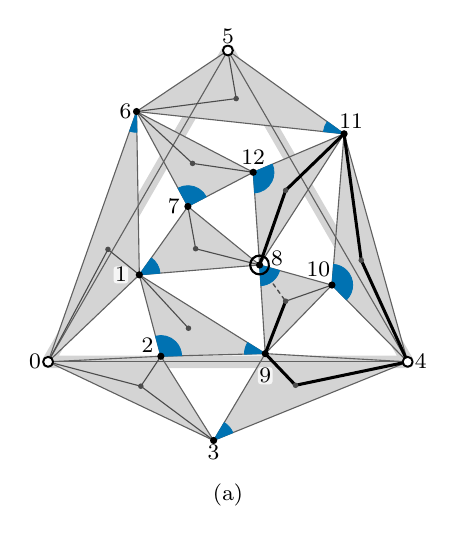
\begin{tikzpicture}[bf,x=0.04348\textwidth,y=0.04348\textwidth]
\draw[bfblack,line width=4.5pt,line join=round] (-4.330,-2.500)--(4.330,-2.500)--(0.000,5.000)--cycle;
\fill[bfblack] (-4.330,-2.500)--(-2.133,-0.405)--(-2.200,3.528)--cycle;
\fill[bfblack] (-4.330,-2.500)--(-1.614,-2.366)--(-0.344,-4.394)--cycle;
\fill[bfblack] (-2.133,-0.405)--(-0.963,1.243)--(0.764,-0.167)--cycle;
\fill[bfblack] (-2.133,-0.405)--(-1.614,-2.366)--(0.900,-2.302)--cycle;
\fill[bfblack] (-0.344,-4.394)--(4.330,-2.500)--(0.900,-2.302)--cycle;
\fill[bfblack] (4.330,-2.500)--(2.506,-0.651)--(2.799,2.992)--cycle;
\fill[bfblack] (0.000,5.000)--(-2.200,3.528)--(2.799,2.992)--cycle;
\fill[bfblack] (-2.200,3.528)--(-0.963,1.243)--(0.610,2.065)--cycle;
\fill[bfblack] (0.764,-0.167)--(2.799,2.992)--(0.610,2.065)--cycle;
\fill[bfblack] (0.764,-0.167)--(0.900,-2.302)--(2.506,-0.651)--cycle;
\draw[bf edge] (-4.330,-2.500)--(-2.133,-0.405);
\draw[bf edge] (-4.330,-2.500)--(-1.614,-2.366);
\draw[bf edge] (-4.330,-2.500)--(-0.344,-4.394);
\draw[bf edge] (-4.330,-2.500)--(4.330,-2.500);
\draw[bf edge] (-4.330,-2.500)--(0.000,5.000);
\draw[bf edge] (-4.330,-2.500)--(-2.200,3.528);
\draw[bf edge] (-2.133,-0.405)--(-1.614,-2.366);
\draw[bf edge] (-2.133,-0.405)--(-2.200,3.528);
\draw[bf edge] (-2.133,-0.405)--(-0.963,1.243);
\draw[bf edge] (-2.133,-0.405)--(0.764,-0.167);
\draw[bf edge] (-2.133,-0.405)--(0.900,-2.302);
\draw[bf edge] (-1.614,-2.366)--(-0.344,-4.394);
\draw[bf edge] (-1.614,-2.366)--(0.900,-2.302);
\draw[bf edge] (-0.344,-4.394)--(4.330,-2.500);
\draw[bf edge] (-0.344,-4.394)--(0.900,-2.302);
\draw[bf edge] (4.330,-2.500)--(0.000,5.000);
\draw[bf edge] (4.330,-2.500)--(0.900,-2.302);
\draw[bf edge] (4.330,-2.500)--(2.506,-0.651);
\draw[bf edge] (4.330,-2.500)--(2.799,2.992);
\draw[bf edge] (0.000,5.000)--(-2.200,3.528);
\draw[bf edge] (0.000,5.000)--(2.799,2.992);
\draw[bf edge] (-2.200,3.528)--(-0.963,1.243);
\draw[bf edge] (-2.200,3.528)--(2.799,2.992);
\draw[bf edge] (-2.200,3.528)--(0.610,2.065);
\draw[bf edge] (-0.963,1.243)--(0.764,-0.167);
\draw[bf edge] (-0.963,1.243)--(0.610,2.065);
\draw[bf edge] (0.764,-0.167)--(0.900,-2.302);
\draw[bf edge] (0.764,-0.167)--(2.506,-0.651);
\draw[bf edge] (0.764,-0.167)--(2.799,2.992);
\draw[bf edge] (0.764,-0.167)--(0.610,2.065);
\draw[bf edge] (0.900,-2.302)--(2.506,-0.651);
\draw[bf edge] (2.506,-0.651)--(2.799,2.992);
\draw[bf edge] (2.799,2.992)--(0.610,2.065);
\draw[bf spoke] (-4.330,-2.500)--(-2.888,0.208);
\draw[bf spoke] (-2.133,-0.405)--(-2.888,0.208);
\draw[bf spoke] (-4.330,-2.500)--(-2.096,-3.087);
\draw[bf spoke] (-1.614,-2.366)--(-2.096,-3.087);
\draw[bf spoke] (-0.344,-4.394)--(-2.096,-3.087);
\draw[bf spoke] (-0.963,1.243)--(-0.777,0.224);
\draw[bf spoke] (0.764,-0.167)--(-0.777,0.224);
\draw[bf spoke] (-2.133,-0.405)--(-0.949,-1.691);
\draw[bf kept] (4.330,-2.500)--(1.629,-3.065);
\draw[bf kept] (0.900,-2.302)--(1.629,-3.065);
\draw[bf kept] (4.330,-2.500)--(3.212,-0.053);
\draw[bf kept] (2.799,2.992)--(3.212,-0.053);
\draw[bf spoke] (0.000,5.000)--(0.200,3.840);
\draw[bf spoke] (-2.200,3.528)--(0.200,3.840);
\draw[bf spoke] (-2.200,3.528)--(-0.851,2.279);
\draw[bf spoke] (0.610,2.065)--(-0.851,2.279);
\draw[bf kept] (0.764,-0.167)--(1.391,1.630);
\draw[bf kept] (2.799,2.992)--(1.391,1.630);
\draw[bf cut] (0.764,-0.167)--(1.390,-1.040);
\draw[bf kept] (0.900,-2.302)--(1.390,-1.040);
\draw[bf spoke] (2.506,-0.651)--(1.390,-1.040);
\path[bf s] (-2.133,-0.405) -- ++(54.6:0.500) arc[start angle=54.6,end angle=4.7,radius=0.500] -- cycle;
\path[bf s] (-1.614,-2.366) -- ++(104.8:0.500) arc[start angle=104.8,end angle=1.5,radius=0.500] -- cycle;
\path[bf s] (-0.344,-4.394) -- ++(22.1:0.500) arc[start angle=22.1,end angle=59.3,radius=0.500] -- cycle;
\path[bf s] (-2.200,3.528) -- ++(-109.5:0.500) arc[start angle=-109.5,end angle=-89.0,radius=0.500] -- cycle;
\path[bf s] (-0.963,1.243) -- ++(118.4:0.500) arc[start angle=118.4,end angle=27.6,radius=0.500] -- cycle;
\path[bf s] (0.764,-0.167) -- ++(-86.4:0.500) arc[start angle=-86.4,end angle=-15.5,radius=0.500] -- cycle;
\path[bf s] (0.900,-2.302) -- ++(148.0:0.500) arc[start angle=148.0,end angle=181.5,radius=0.500] -- cycle;
\path[bf s] (2.506,-0.651) -- ++(-45.4:0.500) arc[start angle=-45.4,end angle=85.4,radius=0.500] -- cycle;
\path[bf s] (2.799,2.992) -- ++(144.3:0.500) arc[start angle=144.3,end angle=173.9,radius=0.500] -- cycle;
\path[bf s] (0.610,2.065) -- ++(-86.1:0.500) arc[start angle=-86.1,end angle=23.0,radius=0.500] -- cycle;
\path[bf root] (-4.330,-2.500) circle[radius=1.8pt];
\path[bf vertex] (-2.133,-0.405) circle[radius=1.3pt];
\path[bf vertex] (-1.614,-2.366) circle[radius=1.3pt];
\path[bf vertex] (-0.344,-4.394) circle[radius=1.3pt];
\path[bf root] (4.330,-2.500) circle[radius=1.8pt];
\path[bf root] (0.000,5.000) circle[radius=1.8pt];
\path[bf vertex] (-2.200,3.528) circle[radius=1.3pt];
\path[bf vertex] (-0.963,1.243) circle[radius=1.3pt];
\path[bf vertex] (0.764,-0.167) circle[radius=1.3pt];
\path[bf vertex] (0.900,-2.302) circle[radius=1.3pt];
\path[bf vertex] (2.506,-0.651) circle[radius=1.3pt];
\path[bf vertex] (2.799,2.992) circle[radius=1.3pt];
\path[bf vertex] (0.610,2.065) circle[radius=1.3pt];
\path[fill=black!70] (-2.888,0.208) circle[radius=1pt];
\path[fill=black!70] (-2.096,-3.087) circle[radius=1pt];
\path[fill=black!70] (-0.777,0.224) circle[radius=1pt];
\path[fill=black!70] (-0.949,-1.691) circle[radius=1pt];
\path[fill=black!70] (1.629,-3.065) circle[radius=1pt];
\path[fill=black!70] (3.212,-0.053) circle[radius=1pt];
\path[fill=black!70] (0.200,3.840) circle[radius=1pt];
\path[fill=black!70] (-0.851,2.279) circle[radius=1pt];
\path[fill=black!70] (1.391,1.630) circle[radius=1pt];
\path[fill=black!70] (1.390,-1.040) circle[radius=1pt];
\draw[draw=black,line width=.8pt] (0.764,-0.167) circle[radius=3.4pt];
\node[fill=white,fill opacity=.8,text opacity=1,inner sep=.5pt,rounded corners=1pt] at (-4.647,-2.500) {$0$};
\node[fill=white,fill opacity=.8,text opacity=1,inner sep=.5pt,rounded corners=1pt] at (-2.577,-0.405) {$1$};
\node[fill=white,fill opacity=.8,text opacity=1,inner sep=.5pt,rounded corners=1pt] at (-1.935,-2.097) {$2$};
\node[fill=white,fill opacity=.8,text opacity=1,inner sep=.5pt,rounded corners=1pt] at (-0.344,-4.686) {$3$};
\node[fill=white,fill opacity=.8,text opacity=1,inner sep=.5pt,rounded corners=1pt] at (4.647,-2.500) {$4$};
\node[fill=white,fill opacity=.8,text opacity=1,inner sep=.5pt,rounded corners=1pt] at (0.000,5.343) {$5$};
\node[fill=white,fill opacity=.8,text opacity=1,inner sep=.5pt,rounded corners=1pt] at (-2.467,3.528) {$6$};
\node[fill=white,fill opacity=.8,text opacity=1,inner sep=.5pt,rounded corners=1pt] at (-1.306,1.243) {$7$};
\node[fill=white,fill opacity=.8,text opacity=1,inner sep=.5pt,rounded corners=1pt] at (1.181,-0.015) {$8$};
\node[fill=white,fill opacity=.8,text opacity=1,inner sep=.5pt,rounded corners=1pt] at (0.900,-2.835) {$9$};
\node[fill=white,fill opacity=.8,text opacity=1,inner sep=.5pt,rounded corners=1pt] at (2.180,-0.262) {$10$};
\node[fill=white,fill opacity=.8,text opacity=1,inner sep=.5pt,rounded corners=1pt] at (2.970,3.289) {$11$};
\node[fill=white,fill opacity=.8,text opacity=1,inner sep=.5pt,rounded corners=1pt] at (0.610,2.433) {$12$};
\node[anchor=north] at (0.000,-5.344) {(a)};
\end{tikzpicture}%
\hspace{0.04\textwidth}%
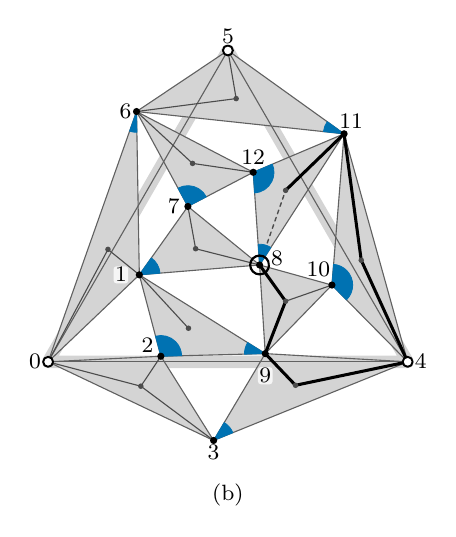
\begin{tikzpicture}[bf,x=0.04348\textwidth,y=0.04348\textwidth]
\draw[bfblack,line width=4.5pt,line join=round] (-4.330,-2.500)--(4.330,-2.500)--(0.000,5.000)--cycle;
\fill[bfblack] (-4.330,-2.500)--(-2.133,-0.405)--(-2.200,3.528)--cycle;
\fill[bfblack] (-4.330,-2.500)--(-1.614,-2.366)--(-0.344,-4.394)--cycle;
\fill[bfblack] (-2.133,-0.405)--(-0.963,1.243)--(0.764,-0.167)--cycle;
\fill[bfblack] (-2.133,-0.405)--(-1.614,-2.366)--(0.900,-2.302)--cycle;
\fill[bfblack] (-0.344,-4.394)--(4.330,-2.500)--(0.900,-2.302)--cycle;
\fill[bfblack] (4.330,-2.500)--(2.506,-0.651)--(2.799,2.992)--cycle;
\fill[bfblack] (0.000,5.000)--(-2.200,3.528)--(2.799,2.992)--cycle;
\fill[bfblack] (-2.200,3.528)--(-0.963,1.243)--(0.610,2.065)--cycle;
\fill[bfblack] (0.764,-0.167)--(2.799,2.992)--(0.610,2.065)--cycle;
\fill[bfblack] (0.764,-0.167)--(0.900,-2.302)--(2.506,-0.651)--cycle;
\draw[bf edge] (-4.330,-2.500)--(-2.133,-0.405);
\draw[bf edge] (-4.330,-2.500)--(-1.614,-2.366);
\draw[bf edge] (-4.330,-2.500)--(-0.344,-4.394);
\draw[bf edge] (-4.330,-2.500)--(4.330,-2.500);
\draw[bf edge] (-4.330,-2.500)--(0.000,5.000);
\draw[bf edge] (-4.330,-2.500)--(-2.200,3.528);
\draw[bf edge] (-2.133,-0.405)--(-1.614,-2.366);
\draw[bf edge] (-2.133,-0.405)--(-2.200,3.528);
\draw[bf edge] (-2.133,-0.405)--(-0.963,1.243);
\draw[bf edge] (-2.133,-0.405)--(0.764,-0.167);
\draw[bf edge] (-2.133,-0.405)--(0.900,-2.302);
\draw[bf edge] (-1.614,-2.366)--(-0.344,-4.394);
\draw[bf edge] (-1.614,-2.366)--(0.900,-2.302);
\draw[bf edge] (-0.344,-4.394)--(4.330,-2.500);
\draw[bf edge] (-0.344,-4.394)--(0.900,-2.302);
\draw[bf edge] (4.330,-2.500)--(0.000,5.000);
\draw[bf edge] (4.330,-2.500)--(0.900,-2.302);
\draw[bf edge] (4.330,-2.500)--(2.506,-0.651);
\draw[bf edge] (4.330,-2.500)--(2.799,2.992);
\draw[bf edge] (0.000,5.000)--(-2.200,3.528);
\draw[bf edge] (0.000,5.000)--(2.799,2.992);
\draw[bf edge] (-2.200,3.528)--(-0.963,1.243);
\draw[bf edge] (-2.200,3.528)--(2.799,2.992);
\draw[bf edge] (-2.200,3.528)--(0.610,2.065);
\draw[bf edge] (-0.963,1.243)--(0.764,-0.167);
\draw[bf edge] (-0.963,1.243)--(0.610,2.065);
\draw[bf edge] (0.764,-0.167)--(0.900,-2.302);
\draw[bf edge] (0.764,-0.167)--(2.506,-0.651);
\draw[bf edge] (0.764,-0.167)--(2.799,2.992);
\draw[bf edge] (0.764,-0.167)--(0.610,2.065);
\draw[bf edge] (0.900,-2.302)--(2.506,-0.651);
\draw[bf edge] (2.506,-0.651)--(2.799,2.992);
\draw[bf edge] (2.799,2.992)--(0.610,2.065);
\draw[bf spoke] (-4.330,-2.500)--(-2.888,0.208);
\draw[bf spoke] (-2.133,-0.405)--(-2.888,0.208);
\draw[bf spoke] (-4.330,-2.500)--(-2.096,-3.087);
\draw[bf spoke] (-1.614,-2.366)--(-2.096,-3.087);
\draw[bf spoke] (-0.344,-4.394)--(-2.096,-3.087);
\draw[bf spoke] (-0.963,1.243)--(-0.777,0.224);
\draw[bf spoke] (0.764,-0.167)--(-0.777,0.224);
\draw[bf spoke] (-2.133,-0.405)--(-0.949,-1.691);
\draw[bf kept] (4.330,-2.500)--(1.629,-3.065);
\draw[bf kept] (0.900,-2.302)--(1.629,-3.065);
\draw[bf kept] (4.330,-2.500)--(3.212,-0.053);
\draw[bf kept] (2.799,2.992)--(3.212,-0.053);
\draw[bf spoke] (0.000,5.000)--(0.200,3.840);
\draw[bf spoke] (-2.200,3.528)--(0.200,3.840);
\draw[bf spoke] (-2.200,3.528)--(-0.851,2.279);
\draw[bf spoke] (0.610,2.065)--(-0.851,2.279);
\draw[bf cut] (0.764,-0.167)--(1.391,1.630);
\draw[bf kept] (2.799,2.992)--(1.391,1.630);
\draw[bf kept] (0.764,-0.167)--(1.390,-1.040);
\draw[bf kept] (0.900,-2.302)--(1.390,-1.040);
\draw[bf spoke] (2.506,-0.651)--(1.390,-1.040);
\path[bf s] (-2.133,-0.405) -- ++(54.6:0.500) arc[start angle=54.6,end angle=4.7,radius=0.500] -- cycle;
\path[bf s] (-1.614,-2.366) -- ++(104.8:0.500) arc[start angle=104.8,end angle=1.5,radius=0.500] -- cycle;
\path[bf s] (-0.344,-4.394) -- ++(22.1:0.500) arc[start angle=22.1,end angle=59.3,radius=0.500] -- cycle;
\path[bf s] (-2.200,3.528) -- ++(-109.5:0.500) arc[start angle=-109.5,end angle=-89.0,radius=0.500] -- cycle;
\path[bf s] (-0.963,1.243) -- ++(118.4:0.500) arc[start angle=118.4,end angle=27.6,radius=0.500] -- cycle;
\path[bf s] (0.764,-0.167) -- ++(57.2:0.500) arc[start angle=57.2,end angle=93.9,radius=0.500] -- cycle;
\path[bf s] (0.900,-2.302) -- ++(148.0:0.500) arc[start angle=148.0,end angle=181.5,radius=0.500] -- cycle;
\path[bf s] (2.506,-0.651) -- ++(-45.4:0.500) arc[start angle=-45.4,end angle=85.4,radius=0.500] -- cycle;
\path[bf s] (2.799,2.992) -- ++(144.3:0.500) arc[start angle=144.3,end angle=173.9,radius=0.500] -- cycle;
\path[bf s] (0.610,2.065) -- ++(-86.1:0.500) arc[start angle=-86.1,end angle=23.0,radius=0.500] -- cycle;
\path[bf root] (-4.330,-2.500) circle[radius=1.8pt];
\path[bf vertex] (-2.133,-0.405) circle[radius=1.3pt];
\path[bf vertex] (-1.614,-2.366) circle[radius=1.3pt];
\path[bf vertex] (-0.344,-4.394) circle[radius=1.3pt];
\path[bf root] (4.330,-2.500) circle[radius=1.8pt];
\path[bf root] (0.000,5.000) circle[radius=1.8pt];
\path[bf vertex] (-2.200,3.528) circle[radius=1.3pt];
\path[bf vertex] (-0.963,1.243) circle[radius=1.3pt];
\path[bf vertex] (0.764,-0.167) circle[radius=1.3pt];
\path[bf vertex] (0.900,-2.302) circle[radius=1.3pt];
\path[bf vertex] (2.506,-0.651) circle[radius=1.3pt];
\path[bf vertex] (2.799,2.992) circle[radius=1.3pt];
\path[bf vertex] (0.610,2.065) circle[radius=1.3pt];
\path[fill=black!70] (-2.888,0.208) circle[radius=1pt];
\path[fill=black!70] (-2.096,-3.087) circle[radius=1pt];
\path[fill=black!70] (-0.777,0.224) circle[radius=1pt];
\path[fill=black!70] (-0.949,-1.691) circle[radius=1pt];
\path[fill=black!70] (1.629,-3.065) circle[radius=1pt];
\path[fill=black!70] (3.212,-0.053) circle[radius=1pt];
\path[fill=black!70] (0.200,3.840) circle[radius=1pt];
\path[fill=black!70] (-0.851,2.279) circle[radius=1pt];
\path[fill=black!70] (1.391,1.630) circle[radius=1pt];
\path[fill=black!70] (1.390,-1.040) circle[radius=1pt];
\draw[draw=black,line width=.8pt] (0.764,-0.167) circle[radius=3.4pt];
\node[fill=white,fill opacity=.8,text opacity=1,inner sep=.5pt,rounded corners=1pt] at (-4.647,-2.500) {$0$};
\node[fill=white,fill opacity=.8,text opacity=1,inner sep=.5pt,rounded corners=1pt] at (-2.577,-0.405) {$1$};
\node[fill=white,fill opacity=.8,text opacity=1,inner sep=.5pt,rounded corners=1pt] at (-1.935,-2.097) {$2$};
\node[fill=white,fill opacity=.8,text opacity=1,inner sep=.5pt,rounded corners=1pt] at (-0.344,-4.686) {$3$};
\node[fill=white,fill opacity=.8,text opacity=1,inner sep=.5pt,rounded corners=1pt] at (4.647,-2.500) {$4$};
\node[fill=white,fill opacity=.8,text opacity=1,inner sep=.5pt,rounded corners=1pt] at (0.000,5.343) {$5$};
\node[fill=white,fill opacity=.8,text opacity=1,inner sep=.5pt,rounded corners=1pt] at (-2.467,3.528) {$6$};
\node[fill=white,fill opacity=.8,text opacity=1,inner sep=.5pt,rounded corners=1pt] at (-1.306,1.243) {$7$};
\node[fill=white,fill opacity=.8,text opacity=1,inner sep=.5pt,rounded corners=1pt] at (1.181,-0.015) {$8$};
\node[fill=white,fill opacity=.8,text opacity=1,inner sep=.5pt,rounded corners=1pt] at (0.900,-2.835) {$9$};
\node[fill=white,fill opacity=.8,text opacity=1,inner sep=.5pt,rounded corners=1pt] at (2.180,-0.262) {$10$};
\node[fill=white,fill opacity=.8,text opacity=1,inner sep=.5pt,rounded corners=1pt] at (2.970,3.289) {$11$};
\node[fill=white,fill opacity=.8,text opacity=1,inner sep=.5pt,rounded corners=1pt] at (0.610,2.433) {$12$};
\node[anchor=north] at (0.000,-5.344) {(b)};
\end{tikzpicture}%
\end{minipage}}
\caption{An exchange at the ringed vertex $x=8$. Thin lines are the arcs of $H_\sigma$, the three arcs at $p_{t_0}$ being omitted, and wedges mark the removed arcs. (a) The rainbow tree of Figure~\ref{fig:rainbow}(a). Adding the removed arc at $8$, dotted, closes the cycle $L$, drawn bold, through the points of the faces $\{8,11,12\}$, $\{4,10,11\}$, $\{3,4,9\}$ and $\{8,9,10\}$. (b) Removing the other arc of $L$ at $8$ moves $8$ from $\{8,9,10\}$ to $\{8,11,12\}$. Both faces have load $1$ before the move, so the excess rises from $2$ to $4$.}
\label{fig:exchange}
\end{figure}

\begin{theorem}\label{thm:even}
Let $n\ge1$, let $t\in A$, and let $s$ be a good state with inverse $\sigma$.
Move $x_0=s(t)$ to $t_1=\alt_\sigma(x_0)$ and take steps from the walk state $P_1=(\sigma[x_0:=t_1],t_1,x_0)$.
The walk stops, at the inverse of a good state $\iota_t(s)$.
The map $\iota_t$ is an involution on the set of good states and has no fixed point.
So the number of good states is even.
\end{theorem}

\begin{proof}
In $P_1$ the excess is $2$, the face $t$ has load $0$ and $t_1$ has load $2$.
A step that does not stop keeps the excess, so in every walk state reached $t$ is the only face of load $0$.
The walk therefore stops exactly when it moves a vertex into $t$, and then the excess is $0$ and the result is the inverse of a good state by Lemma~\ref{lem:good}.

\emph{The walk stops.}
Suppose that $P_1=\step(P)$ for a walk state $P$.
By Lemma~\ref{lem:reverse}, $\step(\mirror(P_1))=\mirror(P)$ is a walk state.
But the resident of $\mirror(P_1)$ is $x_0$, and its exchange leads back into the face $t$ of load $0$, so this step stops.
Hence $P_1$ is not in the image of $\step$.
An injective map on a finite set cannot return to an earlier element of the forward orbit of an element outside its image.
So the walk $P_1,P_2,\dots$ ends at some $P_k$ whose step stops, with a good state $s'$.

\emph{Involution.}
Start from $s'$ at $t$.
The vertex $s'(t)$ is the resident of $P_k$, and its exchange returns it to the face of $P_k$, so the first walk state is $\mirror(P_k)$.
By Lemma~\ref{lem:reverse} the walk continues with $\mirror(P_{k-1}),\dots,\mirror(P_1)$, and the step from $\mirror(P_1)$ puts $x_0$ into $t$ and stops at $s$.
So $\iota_t(s')=s$.

\emph{No fixed point.}
If $s'=s$, the two walks are the same, so $P_i=\mirror(P_{k+1-i})$ for all $i$.
For odd $k$ the middle walk state would equal its mirror, but the arrival and the resident differ.
For even $k$ the walk states $P_{k/2}$ and $P_{k/2+1}$ would have the same rainbow tree, but every step changes it.
\end{proof}

Figure~\ref{fig:orbit} shows one orbit.
The proof uses no sign and no weight, and of the embedding of $T$ only the graph $\Hp$.
In \cite{Paper} the evenness follows from $Z(1)=0$; here every $t\in A$ gives a pairing of the good states.
Neither argument gives existence.
With \cite[Proposition~6.9]{Paper}, a triangulation that has a pair has at least two good states.

\begin{figure}[H]
\centering
\scalebox{.9}{\begin{minipage}{\textwidth}\centering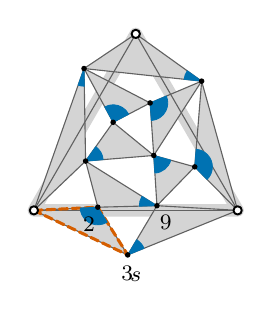
\begin{tikzpicture}[bf,x=0.02464\textwidth,y=0.02464\textwidth]
\draw[bfblack,line width=4.5pt,line join=round] (-4.330,-2.500)--(4.330,-2.500)--(0.000,5.000)--cycle;
\fill[bfblack] (-4.330,-2.500)--(-2.133,-0.405)--(-2.200,3.528)--cycle;
\fill[bfblack] (-4.330,-2.500)--(-1.614,-2.366)--(-0.344,-4.394)--cycle;
\fill[bfblack] (-2.133,-0.405)--(-0.963,1.243)--(0.764,-0.167)--cycle;
\fill[bfblack] (-2.133,-0.405)--(-1.614,-2.366)--(0.900,-2.302)--cycle;
\fill[bfblack] (-0.344,-4.394)--(4.330,-2.500)--(0.900,-2.302)--cycle;
\fill[bfblack] (4.330,-2.500)--(2.506,-0.651)--(2.799,2.992)--cycle;
\fill[bfblack] (0.000,5.000)--(-2.200,3.528)--(2.799,2.992)--cycle;
\fill[bfblack] (-2.200,3.528)--(-0.963,1.243)--(0.610,2.065)--cycle;
\fill[bfblack] (0.764,-0.167)--(2.799,2.992)--(0.610,2.065)--cycle;
\fill[bfblack] (0.764,-0.167)--(0.900,-2.302)--(2.506,-0.651)--cycle;
\draw[bf edge] (-4.330,-2.500)--(-2.133,-0.405);
\draw[bf edge] (-4.330,-2.500)--(-1.614,-2.366);
\draw[bf edge] (-4.330,-2.500)--(-0.344,-4.394);
\draw[bf edge] (-4.330,-2.500)--(4.330,-2.500);
\draw[bf edge] (-4.330,-2.500)--(0.000,5.000);
\draw[bf edge] (-4.330,-2.500)--(-2.200,3.528);
\draw[bf edge] (-2.133,-0.405)--(-1.614,-2.366);
\draw[bf edge] (-2.133,-0.405)--(-2.200,3.528);
\draw[bf edge] (-2.133,-0.405)--(-0.963,1.243);
\draw[bf edge] (-2.133,-0.405)--(0.764,-0.167);
\draw[bf edge] (-2.133,-0.405)--(0.900,-2.302);
\draw[bf edge] (-1.614,-2.366)--(-0.344,-4.394);
\draw[bf edge] (-1.614,-2.366)--(0.900,-2.302);
\draw[bf edge] (-0.344,-4.394)--(4.330,-2.500);
\draw[bf edge] (-0.344,-4.394)--(0.900,-2.302);
\draw[bf edge] (4.330,-2.500)--(0.000,5.000);
\draw[bf edge] (4.330,-2.500)--(0.900,-2.302);
\draw[bf edge] (4.330,-2.500)--(2.506,-0.651);
\draw[bf edge] (4.330,-2.500)--(2.799,2.992);
\draw[bf edge] (0.000,5.000)--(-2.200,3.528);
\draw[bf edge] (0.000,5.000)--(2.799,2.992);
\draw[bf edge] (-2.200,3.528)--(-0.963,1.243);
\draw[bf edge] (-2.200,3.528)--(2.799,2.992);
\draw[bf edge] (-2.200,3.528)--(0.610,2.065);
\draw[bf edge] (-0.963,1.243)--(0.764,-0.167);
\draw[bf edge] (-0.963,1.243)--(0.610,2.065);
\draw[bf edge] (0.764,-0.167)--(0.900,-2.302);
\draw[bf edge] (0.764,-0.167)--(2.506,-0.651);
\draw[bf edge] (0.764,-0.167)--(2.799,2.992);
\draw[bf edge] (0.764,-0.167)--(0.610,2.065);
\draw[bf edge] (0.900,-2.302)--(2.506,-0.651);
\draw[bf edge] (2.506,-0.651)--(2.799,2.992);
\draw[bf edge] (2.799,2.992)--(0.610,2.065);
\draw[bf Q] (-4.330,-2.500)--(-1.614,-2.366)--(-0.344,-4.394)--cycle;
\path[bf s] (-2.133,-0.405) -- ++(54.6:0.750) arc[start angle=54.6,end angle=4.7,radius=0.750] -- cycle;
\path[bf s] (-1.614,-2.366) -- ++(-177.2:0.750) arc[start angle=-177.2,end angle=-57.9,radius=0.750] -- cycle;
\path[bf s] (-0.344,-4.394) -- ++(22.1:0.750) arc[start angle=22.1,end angle=59.3,radius=0.750] -- cycle;
\path[bf s] (-2.200,3.528) -- ++(-109.5:0.750) arc[start angle=-109.5,end angle=-89.0,radius=0.750] -- cycle;
\path[bf s] (-0.963,1.243) -- ++(118.4:0.745) arc[start angle=118.4,end angle=27.6,radius=0.745] -- cycle;
\path[bf s] (0.764,-0.167) -- ++(-86.4:0.750) arc[start angle=-86.4,end angle=-15.5,radius=0.750] -- cycle;
\path[bf s] (0.900,-2.302) -- ++(148.0:0.750) arc[start angle=148.0,end angle=181.5,radius=0.750] -- cycle;
\path[bf s] (2.506,-0.651) -- ++(-45.4:0.750) arc[start angle=-45.4,end angle=85.4,radius=0.750] -- cycle;
\path[bf s] (2.799,2.992) -- ++(144.3:0.750) arc[start angle=144.3,end angle=173.9,radius=0.750] -- cycle;
\path[bf s] (0.610,2.065) -- ++(-86.1:0.750) arc[start angle=-86.1,end angle=23.0,radius=0.750] -- cycle;
\path[bf root] (-4.330,-2.500) circle[radius=1.5pt];
\path[bf vertex] (-2.133,-0.405) circle[radius=1.0pt];
\path[bf vertex] (-1.614,-2.366) circle[radius=1.0pt];
\path[bf vertex] (-0.344,-4.394) circle[radius=1.0pt];
\path[bf root] (4.330,-2.500) circle[radius=1.5pt];
\path[bf root] (0.000,5.000) circle[radius=1.5pt];
\path[bf vertex] (-2.200,3.528) circle[radius=1.0pt];
\path[bf vertex] (-0.963,1.243) circle[radius=1.0pt];
\path[bf vertex] (0.764,-0.167) circle[radius=1.0pt];
\path[bf vertex] (0.900,-2.302) circle[radius=1.0pt];
\path[bf vertex] (2.506,-0.651) circle[radius=1.0pt];
\path[bf vertex] (2.799,2.992) circle[radius=1.0pt];
\path[bf vertex] (0.610,2.065) circle[radius=1.0pt];
\node at (-1.984,-3.075) {$2$};
\node at (-0.367,-5.194) {$3$};
\node at (1.275,-3.008) {$9$};
\node[anchor=north] at (0.000,-4.944) {$s$};
\end{tikzpicture}%
\hfill%
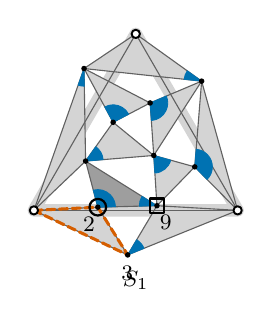
\begin{tikzpicture}[bf,x=0.02464\textwidth,y=0.02464\textwidth]
\draw[bfblack,line width=4.5pt,line join=round] (-4.330,-2.500)--(4.330,-2.500)--(0.000,5.000)--cycle;
\fill[bfblack] (-4.330,-2.500)--(-2.133,-0.405)--(-2.200,3.528)--cycle;
\fill[bfblack] (-4.330,-2.500)--(-1.614,-2.366)--(-0.344,-4.394)--cycle;
\fill[bfblack] (-2.133,-0.405)--(-0.963,1.243)--(0.764,-0.167)--cycle;
\fill[bfblack] (-2.133,-0.405)--(-1.614,-2.366)--(0.900,-2.302)--cycle;
\fill[bfblack] (-0.344,-4.394)--(4.330,-2.500)--(0.900,-2.302)--cycle;
\fill[bfblack] (4.330,-2.500)--(2.506,-0.651)--(2.799,2.992)--cycle;
\fill[bfblack] (0.000,5.000)--(-2.200,3.528)--(2.799,2.992)--cycle;
\fill[bfblack] (-2.200,3.528)--(-0.963,1.243)--(0.610,2.065)--cycle;
\fill[bfblack] (0.764,-0.167)--(2.799,2.992)--(0.610,2.065)--cycle;
\fill[bfblack] (0.764,-0.167)--(0.900,-2.302)--(2.506,-0.651)--cycle;
\fill[black!38] (-2.133,-0.405)--(-1.614,-2.366)--(0.900,-2.302)--cycle;
\draw[bf edge] (-4.330,-2.500)--(-2.133,-0.405);
\draw[bf edge] (-4.330,-2.500)--(-1.614,-2.366);
\draw[bf edge] (-4.330,-2.500)--(-0.344,-4.394);
\draw[bf edge] (-4.330,-2.500)--(4.330,-2.500);
\draw[bf edge] (-4.330,-2.500)--(0.000,5.000);
\draw[bf edge] (-4.330,-2.500)--(-2.200,3.528);
\draw[bf edge] (-2.133,-0.405)--(-1.614,-2.366);
\draw[bf edge] (-2.133,-0.405)--(-2.200,3.528);
\draw[bf edge] (-2.133,-0.405)--(-0.963,1.243);
\draw[bf edge] (-2.133,-0.405)--(0.764,-0.167);
\draw[bf edge] (-2.133,-0.405)--(0.900,-2.302);
\draw[bf edge] (-1.614,-2.366)--(-0.344,-4.394);
\draw[bf edge] (-1.614,-2.366)--(0.900,-2.302);
\draw[bf edge] (-0.344,-4.394)--(4.330,-2.500);
\draw[bf edge] (-0.344,-4.394)--(0.900,-2.302);
\draw[bf edge] (4.330,-2.500)--(0.000,5.000);
\draw[bf edge] (4.330,-2.500)--(0.900,-2.302);
\draw[bf edge] (4.330,-2.500)--(2.506,-0.651);
\draw[bf edge] (4.330,-2.500)--(2.799,2.992);
\draw[bf edge] (0.000,5.000)--(-2.200,3.528);
\draw[bf edge] (0.000,5.000)--(2.799,2.992);
\draw[bf edge] (-2.200,3.528)--(-0.963,1.243);
\draw[bf edge] (-2.200,3.528)--(2.799,2.992);
\draw[bf edge] (-2.200,3.528)--(0.610,2.065);
\draw[bf edge] (-0.963,1.243)--(0.764,-0.167);
\draw[bf edge] (-0.963,1.243)--(0.610,2.065);
\draw[bf edge] (0.764,-0.167)--(0.900,-2.302);
\draw[bf edge] (0.764,-0.167)--(2.506,-0.651);
\draw[bf edge] (0.764,-0.167)--(2.799,2.992);
\draw[bf edge] (0.764,-0.167)--(0.610,2.065);
\draw[bf edge] (0.900,-2.302)--(2.506,-0.651);
\draw[bf edge] (2.506,-0.651)--(2.799,2.992);
\draw[bf edge] (2.799,2.992)--(0.610,2.065);
\draw[bf Q] (-4.330,-2.500)--(-1.614,-2.366)--(-0.344,-4.394)--cycle;
\path[bf s] (-2.133,-0.405) -- ++(54.6:0.750) arc[start angle=54.6,end angle=4.7,radius=0.750] -- cycle;
\path[bf s] (-1.614,-2.366) -- ++(104.8:0.750) arc[start angle=104.8,end angle=1.5,radius=0.750] -- cycle;
\path[bf s] (-0.344,-4.394) -- ++(22.1:0.750) arc[start angle=22.1,end angle=59.3,radius=0.750] -- cycle;
\path[bf s] (-2.200,3.528) -- ++(-109.5:0.750) arc[start angle=-109.5,end angle=-89.0,radius=0.750] -- cycle;
\path[bf s] (-0.963,1.243) -- ++(118.4:0.745) arc[start angle=118.4,end angle=27.6,radius=0.745] -- cycle;
\path[bf s] (0.764,-0.167) -- ++(-86.4:0.750) arc[start angle=-86.4,end angle=-15.5,radius=0.750] -- cycle;
\path[bf s] (0.900,-2.302) -- ++(148.0:0.750) arc[start angle=148.0,end angle=181.5,radius=0.750] -- cycle;
\path[bf s] (2.506,-0.651) -- ++(-45.4:0.750) arc[start angle=-45.4,end angle=85.4,radius=0.750] -- cycle;
\path[bf s] (2.799,2.992) -- ++(144.3:0.750) arc[start angle=144.3,end angle=173.9,radius=0.750] -- cycle;
\path[bf s] (0.610,2.065) -- ++(-86.1:0.750) arc[start angle=-86.1,end angle=23.0,radius=0.750] -- cycle;
\path[bf root] (-4.330,-2.500) circle[radius=1.5pt];
\path[bf vertex] (-2.133,-0.405) circle[radius=1.0pt];
\path[bf vertex] (-1.614,-2.366) circle[radius=1.0pt];
\path[bf vertex] (-0.344,-4.394) circle[radius=1.0pt];
\path[bf root] (4.330,-2.500) circle[radius=1.5pt];
\path[bf root] (0.000,5.000) circle[radius=1.5pt];
\path[bf vertex] (-2.200,3.528) circle[radius=1.0pt];
\path[bf vertex] (-0.963,1.243) circle[radius=1.0pt];
\path[bf vertex] (0.764,-0.167) circle[radius=1.0pt];
\path[bf vertex] (0.900,-2.302) circle[radius=1.0pt];
\path[bf vertex] (2.506,-0.651) circle[radius=1.0pt];
\path[bf vertex] (2.799,2.992) circle[radius=1.0pt];
\path[bf vertex] (0.610,2.065) circle[radius=1.0pt];
\draw[draw=black,line width=.8pt] (-1.614,-2.366) circle[radius=3.0pt];
\draw[draw=black,line width=.8pt] (0.900,-2.302) +(-2.6pt,-2.6pt) rectangle +(2.6pt,2.6pt);
\node at (-1.984,-3.075) {$2$};
\node at (-0.367,-5.194) {$3$};
\node at (1.275,-3.008) {$9$};
\node[anchor=north] at (0.000,-4.944) {$S_1$};
\end{tikzpicture}%
\hfill%
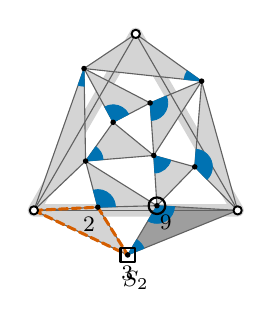
\begin{tikzpicture}[bf,x=0.02464\textwidth,y=0.02464\textwidth]
\draw[bfblack,line width=4.5pt,line join=round] (-4.330,-2.500)--(4.330,-2.500)--(0.000,5.000)--cycle;
\fill[bfblack] (-4.330,-2.500)--(-2.133,-0.405)--(-2.200,3.528)--cycle;
\fill[bfblack] (-4.330,-2.500)--(-1.614,-2.366)--(-0.344,-4.394)--cycle;
\fill[bfblack] (-2.133,-0.405)--(-0.963,1.243)--(0.764,-0.167)--cycle;
\fill[bfblack] (-2.133,-0.405)--(-1.614,-2.366)--(0.900,-2.302)--cycle;
\fill[bfblack] (-0.344,-4.394)--(4.330,-2.500)--(0.900,-2.302)--cycle;
\fill[bfblack] (4.330,-2.500)--(2.506,-0.651)--(2.799,2.992)--cycle;
\fill[bfblack] (0.000,5.000)--(-2.200,3.528)--(2.799,2.992)--cycle;
\fill[bfblack] (-2.200,3.528)--(-0.963,1.243)--(0.610,2.065)--cycle;
\fill[bfblack] (0.764,-0.167)--(2.799,2.992)--(0.610,2.065)--cycle;
\fill[bfblack] (0.764,-0.167)--(0.900,-2.302)--(2.506,-0.651)--cycle;
\fill[black!38] (-0.344,-4.394)--(4.330,-2.500)--(0.900,-2.302)--cycle;
\draw[bf edge] (-4.330,-2.500)--(-2.133,-0.405);
\draw[bf edge] (-4.330,-2.500)--(-1.614,-2.366);
\draw[bf edge] (-4.330,-2.500)--(-0.344,-4.394);
\draw[bf edge] (-4.330,-2.500)--(4.330,-2.500);
\draw[bf edge] (-4.330,-2.500)--(0.000,5.000);
\draw[bf edge] (-4.330,-2.500)--(-2.200,3.528);
\draw[bf edge] (-2.133,-0.405)--(-1.614,-2.366);
\draw[bf edge] (-2.133,-0.405)--(-2.200,3.528);
\draw[bf edge] (-2.133,-0.405)--(-0.963,1.243);
\draw[bf edge] (-2.133,-0.405)--(0.764,-0.167);
\draw[bf edge] (-2.133,-0.405)--(0.900,-2.302);
\draw[bf edge] (-1.614,-2.366)--(-0.344,-4.394);
\draw[bf edge] (-1.614,-2.366)--(0.900,-2.302);
\draw[bf edge] (-0.344,-4.394)--(4.330,-2.500);
\draw[bf edge] (-0.344,-4.394)--(0.900,-2.302);
\draw[bf edge] (4.330,-2.500)--(0.000,5.000);
\draw[bf edge] (4.330,-2.500)--(0.900,-2.302);
\draw[bf edge] (4.330,-2.500)--(2.506,-0.651);
\draw[bf edge] (4.330,-2.500)--(2.799,2.992);
\draw[bf edge] (0.000,5.000)--(-2.200,3.528);
\draw[bf edge] (0.000,5.000)--(2.799,2.992);
\draw[bf edge] (-2.200,3.528)--(-0.963,1.243);
\draw[bf edge] (-2.200,3.528)--(2.799,2.992);
\draw[bf edge] (-2.200,3.528)--(0.610,2.065);
\draw[bf edge] (-0.963,1.243)--(0.764,-0.167);
\draw[bf edge] (-0.963,1.243)--(0.610,2.065);
\draw[bf edge] (0.764,-0.167)--(0.900,-2.302);
\draw[bf edge] (0.764,-0.167)--(2.506,-0.651);
\draw[bf edge] (0.764,-0.167)--(2.799,2.992);
\draw[bf edge] (0.764,-0.167)--(0.610,2.065);
\draw[bf edge] (0.900,-2.302)--(2.506,-0.651);
\draw[bf edge] (2.506,-0.651)--(2.799,2.992);
\draw[bf edge] (2.799,2.992)--(0.610,2.065);
\draw[bf Q] (-4.330,-2.500)--(-1.614,-2.366)--(-0.344,-4.394)--cycle;
\path[bf s] (-2.133,-0.405) -- ++(54.6:0.750) arc[start angle=54.6,end angle=4.7,radius=0.750] -- cycle;
\path[bf s] (-1.614,-2.366) -- ++(104.8:0.750) arc[start angle=104.8,end angle=1.5,radius=0.750] -- cycle;
\path[bf s] (-0.344,-4.394) -- ++(22.1:0.750) arc[start angle=22.1,end angle=59.3,radius=0.750] -- cycle;
\path[bf s] (-2.200,3.528) -- ++(-109.5:0.750) arc[start angle=-109.5,end angle=-89.0,radius=0.750] -- cycle;
\path[bf s] (-0.963,1.243) -- ++(118.4:0.745) arc[start angle=118.4,end angle=27.6,radius=0.745] -- cycle;
\path[bf s] (0.764,-0.167) -- ++(-86.4:0.750) arc[start angle=-86.4,end angle=-15.5,radius=0.750] -- cycle;
\path[bf s] (0.900,-2.302) -- ++(-120.7:0.750) arc[start angle=-120.7,end angle=-3.3,radius=0.750] -- cycle;
\path[bf s] (2.506,-0.651) -- ++(-45.4:0.750) arc[start angle=-45.4,end angle=85.4,radius=0.750] -- cycle;
\path[bf s] (2.799,2.992) -- ++(144.3:0.750) arc[start angle=144.3,end angle=173.9,radius=0.750] -- cycle;
\path[bf s] (0.610,2.065) -- ++(-86.1:0.750) arc[start angle=-86.1,end angle=23.0,radius=0.750] -- cycle;
\path[bf root] (-4.330,-2.500) circle[radius=1.5pt];
\path[bf vertex] (-2.133,-0.405) circle[radius=1.0pt];
\path[bf vertex] (-1.614,-2.366) circle[radius=1.0pt];
\path[bf vertex] (-0.344,-4.394) circle[radius=1.0pt];
\path[bf root] (4.330,-2.500) circle[radius=1.5pt];
\path[bf root] (0.000,5.000) circle[radius=1.5pt];
\path[bf vertex] (-2.200,3.528) circle[radius=1.0pt];
\path[bf vertex] (-0.963,1.243) circle[radius=1.0pt];
\path[bf vertex] (0.764,-0.167) circle[radius=1.0pt];
\path[bf vertex] (0.900,-2.302) circle[radius=1.0pt];
\path[bf vertex] (2.506,-0.651) circle[radius=1.0pt];
\path[bf vertex] (2.799,2.992) circle[radius=1.0pt];
\path[bf vertex] (0.610,2.065) circle[radius=1.0pt];
\draw[draw=black,line width=.8pt] (0.900,-2.302) circle[radius=3.0pt];
\draw[draw=black,line width=.8pt] (-0.344,-4.394) +(-2.6pt,-2.6pt) rectangle +(2.6pt,2.6pt);
\node at (-1.984,-3.075) {$2$};
\node at (-0.367,-5.194) {$3$};
\node at (1.275,-3.008) {$9$};
\node[anchor=north] at (0.000,-4.944) {$S_2$};
\end{tikzpicture}%
\hfill%
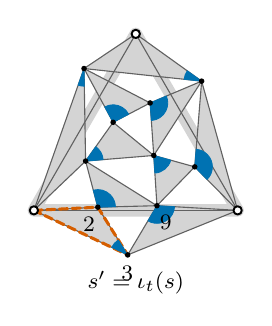
\begin{tikzpicture}[bf,x=0.02464\textwidth,y=0.02464\textwidth]
\draw[bfblack,line width=4.5pt,line join=round] (-4.330,-2.500)--(4.330,-2.500)--(0.000,5.000)--cycle;
\fill[bfblack] (-4.330,-2.500)--(-2.133,-0.405)--(-2.200,3.528)--cycle;
\fill[bfblack] (-4.330,-2.500)--(-1.614,-2.366)--(-0.344,-4.394)--cycle;
\fill[bfblack] (-2.133,-0.405)--(-0.963,1.243)--(0.764,-0.167)--cycle;
\fill[bfblack] (-2.133,-0.405)--(-1.614,-2.366)--(0.900,-2.302)--cycle;
\fill[bfblack] (-0.344,-4.394)--(4.330,-2.500)--(0.900,-2.302)--cycle;
\fill[bfblack] (4.330,-2.500)--(2.506,-0.651)--(2.799,2.992)--cycle;
\fill[bfblack] (0.000,5.000)--(-2.200,3.528)--(2.799,2.992)--cycle;
\fill[bfblack] (-2.200,3.528)--(-0.963,1.243)--(0.610,2.065)--cycle;
\fill[bfblack] (0.764,-0.167)--(2.799,2.992)--(0.610,2.065)--cycle;
\fill[bfblack] (0.764,-0.167)--(0.900,-2.302)--(2.506,-0.651)--cycle;
\draw[bf edge] (-4.330,-2.500)--(-2.133,-0.405);
\draw[bf edge] (-4.330,-2.500)--(-1.614,-2.366);
\draw[bf edge] (-4.330,-2.500)--(-0.344,-4.394);
\draw[bf edge] (-4.330,-2.500)--(4.330,-2.500);
\draw[bf edge] (-4.330,-2.500)--(0.000,5.000);
\draw[bf edge] (-4.330,-2.500)--(-2.200,3.528);
\draw[bf edge] (-2.133,-0.405)--(-1.614,-2.366);
\draw[bf edge] (-2.133,-0.405)--(-2.200,3.528);
\draw[bf edge] (-2.133,-0.405)--(-0.963,1.243);
\draw[bf edge] (-2.133,-0.405)--(0.764,-0.167);
\draw[bf edge] (-2.133,-0.405)--(0.900,-2.302);
\draw[bf edge] (-1.614,-2.366)--(-0.344,-4.394);
\draw[bf edge] (-1.614,-2.366)--(0.900,-2.302);
\draw[bf edge] (-0.344,-4.394)--(4.330,-2.500);
\draw[bf edge] (-0.344,-4.394)--(0.900,-2.302);
\draw[bf edge] (4.330,-2.500)--(0.000,5.000);
\draw[bf edge] (4.330,-2.500)--(0.900,-2.302);
\draw[bf edge] (4.330,-2.500)--(2.506,-0.651);
\draw[bf edge] (4.330,-2.500)--(2.799,2.992);
\draw[bf edge] (0.000,5.000)--(-2.200,3.528);
\draw[bf edge] (0.000,5.000)--(2.799,2.992);
\draw[bf edge] (-2.200,3.528)--(-0.963,1.243);
\draw[bf edge] (-2.200,3.528)--(2.799,2.992);
\draw[bf edge] (-2.200,3.528)--(0.610,2.065);
\draw[bf edge] (-0.963,1.243)--(0.764,-0.167);
\draw[bf edge] (-0.963,1.243)--(0.610,2.065);
\draw[bf edge] (0.764,-0.167)--(0.900,-2.302);
\draw[bf edge] (0.764,-0.167)--(2.506,-0.651);
\draw[bf edge] (0.764,-0.167)--(2.799,2.992);
\draw[bf edge] (0.764,-0.167)--(0.610,2.065);
\draw[bf edge] (0.900,-2.302)--(2.506,-0.651);
\draw[bf edge] (2.506,-0.651)--(2.799,2.992);
\draw[bf edge] (2.799,2.992)--(0.610,2.065);
\draw[bf Q] (-4.330,-2.500)--(-1.614,-2.366)--(-0.344,-4.394)--cycle;
\path[bf s] (-2.133,-0.405) -- ++(54.6:0.750) arc[start angle=54.6,end angle=4.7,radius=0.750] -- cycle;
\path[bf s] (-1.614,-2.366) -- ++(104.8:0.750) arc[start angle=104.8,end angle=1.5,radius=0.750] -- cycle;
\path[bf s] (-0.344,-4.394) -- ++(154.6:0.750) arc[start angle=154.6,end angle=122.1,radius=0.750] -- cycle;
\path[bf s] (-2.200,3.528) -- ++(-109.5:0.750) arc[start angle=-109.5,end angle=-89.0,radius=0.750] -- cycle;
\path[bf s] (-0.963,1.243) -- ++(118.4:0.745) arc[start angle=118.4,end angle=27.6,radius=0.745] -- cycle;
\path[bf s] (0.764,-0.167) -- ++(-86.4:0.750) arc[start angle=-86.4,end angle=-15.5,radius=0.750] -- cycle;
\path[bf s] (0.900,-2.302) -- ++(-120.7:0.750) arc[start angle=-120.7,end angle=-3.3,radius=0.750] -- cycle;
\path[bf s] (2.506,-0.651) -- ++(-45.4:0.750) arc[start angle=-45.4,end angle=85.4,radius=0.750] -- cycle;
\path[bf s] (2.799,2.992) -- ++(144.3:0.750) arc[start angle=144.3,end angle=173.9,radius=0.750] -- cycle;
\path[bf s] (0.610,2.065) -- ++(-86.1:0.750) arc[start angle=-86.1,end angle=23.0,radius=0.750] -- cycle;
\path[bf root] (-4.330,-2.500) circle[radius=1.5pt];
\path[bf vertex] (-2.133,-0.405) circle[radius=1.0pt];
\path[bf vertex] (-1.614,-2.366) circle[radius=1.0pt];
\path[bf vertex] (-0.344,-4.394) circle[radius=1.0pt];
\path[bf root] (4.330,-2.500) circle[radius=1.5pt];
\path[bf root] (0.000,5.000) circle[radius=1.5pt];
\path[bf vertex] (-2.200,3.528) circle[radius=1.0pt];
\path[bf vertex] (-0.963,1.243) circle[radius=1.0pt];
\path[bf vertex] (0.764,-0.167) circle[radius=1.0pt];
\path[bf vertex] (0.900,-2.302) circle[radius=1.0pt];
\path[bf vertex] (2.506,-0.651) circle[radius=1.0pt];
\path[bf vertex] (2.799,2.992) circle[radius=1.0pt];
\path[bf vertex] (0.610,2.065) circle[radius=1.0pt];
\node at (-1.984,-3.075) {$2$};
\node at (-0.367,-5.194) {$3$};
\node at (1.275,-3.008) {$9$};
\node[anchor=north] at (0.000,-4.944) {$s'=\iota_t(s)$};
\end{tikzpicture}%
\end{minipage}}
\caption{One orbit of the involution $\iota_t$ for the face $t=\{0,2,3\}$, dashed outline, in the example. In the good state $s$ the vertex $2$ is $s(t)$. Its exchange moves it to $\{1,2,9\}$, which becomes the face of load $2$, drawn dark, in the walk state $P_1$ with arrival $2$, ringed, and resident $9$, boxed. The rainbow tree of $P_1$ is the one of Figure~\ref{fig:rainbow}(a). The step moves $9$ to $\{3,4,9\}$ and gives $P_2$ with arrival $9$ and resident $3$. The next step moves $3$ into $t$ and stops at the good state $s'$.}
\label{fig:orbit}
\end{figure}

\section{Each condition alone, in every \texorpdfstring{$2$}{2}-factor}\label{sec:packing}

As in \cite[Section~4]{Paper}, for $U\subseteq V(T)$ let $e(U)$ be the number of edges of $T$ with both ends in $U$ and $b(U)$ the number of black faces of $T$, $t_0$ included, with all three corners in $U$.
Let $\rho(U)$ be the number of roots in $U$, and for a black face $t$ write $j_t=|V(t)\cap U|$.
Every edge of $T$ lies on exactly one black face, and a black face with $3,2,1,0$ corners in $U$ has $3,1,0,0$ sides with both ends in $U$, so
\begin{equation}\label{eq:shortfall}
e(U)-b(U)=\sum_{t\ \mathrm{black}}\max(0,j_t-1).
\end{equation}
The next lemma is the computation in the proof of \cite[Lemma~4.4]{Paper}, kept as an identity and without the assumption that $T$ has no separating triangle.

\begin{lemma}\label{lem:identity}
Let $K$ be a connected induced subgraph of $T$ with $p\ge3$ vertices and $q$ edges.
Call a face of the plane graph $K$ a \emph{region} if it is not a face of $T$.
Let $b_K$ be the number of black faces of $T$ with all corners in $K$, and for a region $\Psi$ let $d_\Psi$ be the length of its boundary in edge sides and $\beta_\Psi$ the number of black faces of $T$ contained in $\Psi$ minus the number of white ones.
Then
\[
q-b_K-(2p-4)=\tfrac12\sum_{\Psi}\bigl(\beta_\Psi-d_\Psi+4\bigr),
\]
and $\beta_\Psi\le d_\Psi-4$ if $d_\Psi\ge4$, while $\beta_\Psi=\pm1$ if $d_\Psi=3$, with $+1$ exactly when the three faces of $T$ in $\Psi$ along its boundary are black.
\end{lemma}

\begin{proof}
A face of $T$ with all corners in $K$ is a face of $K$.
Let $w_K$ be the number of white ones and $g$ the number of regions.
Euler's formula $p-q+b_K+w_K+g=2$ and the count of sides $2q=3b_K+3w_K+\sum_\Psi d_\Psi$ give $q-b_K-(2p-4)=\frac12\bigl(w_K-b_K-\sum_\Psi(d_\Psi-4)\bigr)$.
$T$ has as many black faces as white ones, so $w_K-b_K=\sum_\Psi\beta_\Psi$.
As in the proof of Theorem~\ref{thm:R}, $3\beta_\Psi$ is a sum of $d_\Psi$ terms $\pm1$, one for each boundary side.
This gives $\beta_\Psi=\pm1$ for $d_\Psi=3$, $\beta_\Psi=0$ for $d_\Psi=4$, $|\beta_\Psi|\le1$ for $d_\Psi=5$ and $|\beta_\Psi|\le d_\Psi/3\le d_\Psi-4$ for $d_\Psi\ge6$.
\end{proof}

\begin{lemma}\label{lem:density}
Suppose that no separating triangle of $T$ has three black faces along its inner side.
Then for every nonempty $U\subseteq V(T)$
\begin{equation}\label{eq:density}
e(U)-b(U)+\max(0,\rho(U)-1)\ \le\ 2|U|-2 .
\end{equation}
\end{lemma}

For sets $U$ that contain the roots this is the inequality of \cite[Lemma~4.4]{Paper}, under a weaker assumption.

\begin{proof}
Edges and black faces with corners in $U$ lie in one component of $T[U]$, and so do the roots in $U$, which are pairwise adjacent.
Since $\sum_K(2p_K-2)\le2|U|-2$, it suffices to show $q-b_K\le2p-2-\max(0,\rho_K-1)$ for every component $K$ of $T[U]$, with $p$ vertices, $q$ edges and $\rho_K$ roots, and $b_K$ as in Lemma~\ref{lem:identity}.
For $p\le2$ this is clear.
For $p=3$, a path has $q-b_K=2$ and at most two roots.
A triangle that bounds a black face has $q-b_K=2$, and any other triangle has $q-b_K=3$ and at most two roots, because the triangle on the three roots bounds $t_0$.

Let $p\ge4$ and apply Lemma~\ref{lem:identity}.
A region with $d_\Psi\ge4$ contributes at most $0$.
A region with $d_\Psi=3$ is one side of a triangle of $T$.
It contains a vertex of $T$, since it is not a face of $T$, and $K$ has a vertex on the other side.
So the triangle is a separating triangle.
If the region does not contain $t_0$, it is the inner side, so $\beta_\Psi=-1$ by assumption and the contribution is $0$.
At most one region contains $t_0$, and it contributes at most $1$.
Hence $q-b_K\le2p-4+\eta$, where $\eta=1$ if $t_0$ lies in a region with $d_\Psi=3$ and $\eta=0$ otherwise.
If $\rho_K=3$ then $t_0$ is a face of $K$, so $\eta=0$.
If $\rho_K\le2$ then $2p-3\le2p-2-\max(0,\rho_K-1)$.
\end{proof}

We use two theorems on packing.
Nash-Williams \cite{NashWilliams}, \cite[Exercise~10.29]{SchrijverCourse}: the edges of a multigraph without loops can be partitioned into $k$ forests if and only if every nonempty set $Z$ of vertices spans at most $k(|Z|-1)$ edges.
Edmonds \cite{Edmonds}, \cite[pp.~1674 and 1685--1686]{SchrijverHandbook}: in a directed graph with a vertex $\varrho$, the largest number of pairwise arc-disjoint spanning trees directed towards $\varrho$ equals the smallest number of arcs leaving a nonempty set of vertices that does not contain $\varrho$.
(The source states this for trees directed away from $\varrho$; reverse all arcs.)

In the next two theorems $u$ is any map that assigns to every $t\in A$ one of its corners.
Every $2$-factor of $H$ gives such a map, but most such maps come from no $2$-factor.

\begin{theorem}\label{thm:twotrees}
Suppose that no separating triangle of $T$ has three black faces along its inner side, and let $u$ assign to every $t\in A$ one of its corners.
Then the $2n$ edges $(vt)^*$ of $W$ with $t\in A$ and $v\ne u(t)$ can be partitioned into two spanning trees of $W$.
In particular, for every $2$-factor $F$ of $H$ the edges $(xt)^*$ with $xt\in E(F)$ form two spanning trees of $W$.
\end{theorem}

\begin{proof}
Let $M_u$ be the multigraph obtained from $\Hp$ by doubling the three arcs at $p_{t_0}$ and the arcs $u(t)t$, $t\in A$.
It has $6+2n+2n=2(|V(\Hp)|-1)$ edges.
Let $Z$ be a set of vertices of $\Hp$, let $U=Z\cap V(T)$, and let $\mu_t$ be the number of edges of $M_u$ from $p_t$ to $U$.
If $U$ is empty, $Z$ spans no edge.
Otherwise $Z$ spans at most $2(|Z|-1)$ edges, whichever points $p_t$ it contains, exactly when
\begin{equation}\label{eq:nw}
\sum_{t\ \mathrm{black}}\max(0,\mu_t-2)\ \le\ 2|U|-2 .
\end{equation}
For $t_0$ the term is $2\max(0,\rho(U)-1)$.
For $t\in A$ we have $\mu_t=4$ if $j_t=3$, $\mu_t=3$ if $j_t=2$ and $u(t)\in U$, and $\mu_t\le2$ otherwise, so the term is at most $\max(0,j_t-1)$.
By \eqref{eq:shortfall}, in which $t_0$ accounts for $\max(0,\rho(U)-1)$, the left side of \eqref{eq:nw} is at most $e(U)-b(U)+\max(0,\rho(U)-1)$, and Lemma~\ref{lem:density} gives \eqref{eq:nw}.
By the theorem of Nash-Williams, $M_u$ is the union of two forests.
By the count of edges both are spanning trees, and each contains one copy of every doubled arc.
So the complement in $\Hp$ of each of them consists of the arcs that are not doubled and lie in the other, and by Lemma~\ref{lem:dual} the duals of these two sets of arcs are spanning trees of $W$.
\end{proof}

\begin{remark}\label{rem:needed}
The assumption is needed.
Let $\Delta$ be a separating triangle with three black faces $t_1,t_2,t_3$ along its inner side, and let $u(t_i)$ lie on $\Delta$ for each $i$.
For the set $U$ of the vertices that are not on the inner side of $\Delta$, Lemma~\ref{lem:identity} gives $e(U)-b(U)=2|U|-3$, every term of \eqref{eq:nw} equals its bound, and the left side of \eqref{eq:nw} is $2|U|-1$.
So the edges cannot be partitioned in this way.
\end{remark}

\begin{theorem}\label{thm:twoforests}
Suppose that no separating triangle of $T$ has three black faces along its inner side, and let $u$ assign to every $t\in A$ one of its corners.
Then the $2n$ sides of the faces $t\in A$ at the corners $u(t)$ can be partitioned into two spanning forests of $T$, each with three components and one root in each component.
For a pair $(r,s)$ and its third corners $u(t)$, these sides are the edges of $Q_r$ and $Q_s$.
\end{theorem}

\begin{proof}
Identify the three roots to one vertex $\varrho$.
The resulting multigraph $T'$ has $n+1$ vertices, and the $2n$ sides give no loops, because an edge between two roots is a side of $t_0$.
A face $t\in A$ with $j_t$ corners in a set has at most $\max(0,j_t-1)$ of its two sides inside it.
Let $Z$ be a nonempty set of vertices of $T'$.
If $\varrho\notin Z$, then by \eqref{eq:shortfall} and Lemma~\ref{lem:density} the number of sides with both ends in $Z$ is at most $e(Z)-b(Z)\le2|Z|-2$.
If $\varrho\in Z$, let $U$ consist of $Z\setminus\{\varrho\}$ and the three roots, so that $|U|=|Z|+2$; the number of sides is then at most $e(U)-b(U)-2\le2|U|-6=2|Z|-2$.
By the theorem of Nash-Williams the sides form two forests of $T'$, with $2n$ edges, hence two spanning trees.
A spanning tree of $T'$ is a spanning forest of $T$ with one root in each of its three components.
In a pair, the side of $t$ opposite $r(t)$ joins $s(t)$ and $u(t)$, and the side opposite $s(t)$ joins $r(t)$ and $u(t)$.
\end{proof}

\begin{theorem}\label{thm:edmonds}
Suppose that no separating triangle of $T$ has three black faces along its inner side.
Then for every $2$-factor $F$ of $H$ there are two rainbow trees $\sigma$ and $\sigma'$ such that the edges of $F$ are the edges $x\sigma(x)$ and $x\sigma'(x)$, $x\in X$.
\end{theorem}

\begin{proof}
Identify the roots of $D_F$ to one vertex $\varrho$.
By Lemma~\ref{lem:orient}, two rainbow trees $\sigma$ and $\sigma'$ as in the theorem are a partition of the arcs into two spanning trees directed towards $\varrho$.
Conversely two such trees without a common arc have $n$ arcs each, one out of every vertex of $X$, so they contain all arcs and give $\sigma$ and $\sigma'$.
By the theorem of Edmonds they exist if at least two arcs leave every nonempty $Y\subseteq X$.
Every vertex of $Y$ has outdegree two, so this says that at most $2|Y|-2$ arcs have both ends in $Y$.
A face $t$ has such arcs only if $u(t)\in Y$, and then at most $j_t-1$ of them, where $j_t=|V(t)\cap Y|$.
By \eqref{eq:shortfall} and Lemma~\ref{lem:density} with $\rho(Y)=0$ their number is at most $e(Y)-b(Y)\le2|Y|-2$.
\end{proof}

\begin{corollary}\label{cor:alone}
Suppose that no separating triangle of $T$ has three black faces along its inner side, and let $F$ be a $2$-factor of $H$.
Then some spanning tree of $W$ with edges $(xt)^*$, $xt\in E(F)$, satisfies the vertex condition, and some spanning tree of this kind satisfies the face condition.
\end{corollary}

\begin{proof}
The first is Theorem~\ref{thm:edmonds}.
For the second, the $2n$ edges $(xt)^*$ with $xt\in E(F)$ form two forests by Theorem~\ref{thm:twotrees}, so every set $N$ of them has rank at least $|N|/2$.
The $n$ sets $\{(xt)^*:xt\in E(F)\}$, $t\in A$, are disjoint and have two elements each, so the union of any $j$ of them has rank at least $j$.
Rado's theorem gives an independent transversal, which is a spanning tree of $W$ with the face condition.
\end{proof}

\section{Where it stops}\label{sec:wall}

\subsection*{A \texorpdfstring{$2$}{2}-factor without a good state}
A good state in a $2$-factor $F$ is a spanning tree of $W$ with edges $(xt)^*$, $xt\in E(F)$, that satisfies both conditions.
Corollary~\ref{cor:alone} meets each of them alone.
Both together can fail; this is the example mentioned in the Remarks of \cite{Paper}.

\begin{proposition}\label{prop:bad}
Let $T$ be the Eulerian triangulation with $16$ vertices of Figure~\ref{fig:bad}, with $t_0=\{0,1,2\}$.
No separating triangle of $T$ has three black faces along its inner side, $H$ has three $2$-factors, and $T$ has $12$ good states.
One of the $2$-factors, $F$, has a single cycle, and neither of the two pairs with $2$-factor $F$ has a good second state.
There are $6144$ rainbow trees in $F$, all of positive excess.
\end{proposition}

\begin{proof}
The faces in $A$ are, with the corner $u(t)$ for $F$ written first,
\begin{gather*}
(0,3,4),\ (0,5,6),\ (0,7,8),\ (1,8,9),\ (1,10,11),\ (2,3,13),\ (2,11,12),\\
(13,4,5),\ (5,14,15),\ (7,6,15),\ (9,7,14),\ (12,9,10),\ (14,12,13).
\end{gather*}
The sides opposite the corners $u(t)$ form the cycle $3,4,5,6,15,14,7,8,9,10,11,12,13$ through all vertices of $X$, so $F$ has a single cycle and two states lie in $F$.
For one of them $Q_s$ contains the triangle $5,13,14$, and for the other the triangle $9,12,14$.
As $H$ has a $2$-factor, no separating triangle has three black faces along its inner side, by Corollary~\ref{cor:pair}.
The numbers of $2$-factors, good states and rainbow trees are found by enumeration.
\end{proof}

\begin{figure}[H]
\centering
\scalebox{.85}{\begin{minipage}{\textwidth}\centering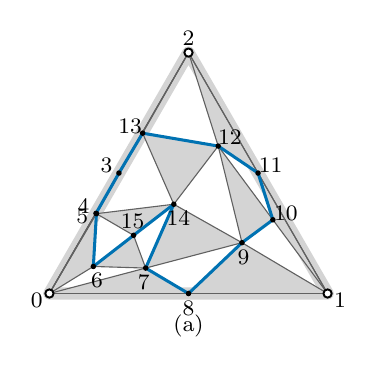
\begin{tikzpicture}[bf,x=0.03364\textwidth,y=0.03364\textwidth]
\draw[bfblack,line width=4.5pt,line join=round] (-4.330,-2.500)--(4.330,-2.500)--(0.000,5.000)--cycle;
\fill[bfblack] (-4.330,-2.500)--(-2.165,1.250)--(-2.879,-0.004)--cycle;
\fill[bfblack] (-4.330,-2.500)--(-2.866,-0.015)--(-2.962,-1.658)--cycle;
\fill[bfblack] (-4.330,-2.500)--(-1.333,-1.708)--(-0.000,-2.500)--cycle;
\fill[bfblack] (4.330,-2.500)--(-0.000,-2.500)--(1.665,-0.918)--cycle;
\fill[bfblack] (4.330,-2.500)--(2.627,-0.205)--(2.165,1.250)--cycle;
\fill[bfblack] (0.000,5.000)--(-2.165,1.250)--(-1.428,2.491)--cycle;
\fill[bfblack] (0.000,5.000)--(2.165,1.250)--(0.925,2.090)--cycle;
\fill[bfblack] (-2.879,-0.004)--(-2.866,-0.015)--(-1.428,2.491)--cycle;
\fill[bfblack] (-2.866,-0.015)--(-0.457,0.279)--(-1.710,-0.689)--cycle;
\fill[bfblack] (-2.962,-1.658)--(-1.333,-1.708)--(-1.710,-0.689)--cycle;
\fill[bfblack] (-1.333,-1.708)--(1.665,-0.918)--(-0.457,0.279)--cycle;
\fill[bfblack] (1.665,-0.918)--(2.627,-0.205)--(0.925,2.090)--cycle;
\fill[bfblack] (0.925,2.090)--(-1.428,2.491)--(-0.457,0.279)--cycle;
\draw[bf edge] (-4.330,-2.500)--(4.330,-2.500);
\draw[bf edge] (-4.330,-2.500)--(0.000,5.000);
\draw[bf edge] (-4.330,-2.500)--(-2.165,1.250);
\draw[bf edge] (-4.330,-2.500)--(-2.879,-0.004);
\draw[bf edge] (-4.330,-2.500)--(-2.866,-0.015);
\draw[bf edge] (-4.330,-2.500)--(-2.962,-1.658);
\draw[bf edge] (-4.330,-2.500)--(-1.333,-1.708);
\draw[bf edge] (-4.330,-2.500)--(-0.000,-2.500);
\draw[bf edge] (4.330,-2.500)--(0.000,5.000);
\draw[bf edge] (4.330,-2.500)--(-0.000,-2.500);
\draw[bf edge] (4.330,-2.500)--(1.665,-0.918);
\draw[bf edge] (4.330,-2.500)--(2.627,-0.205);
\draw[bf edge] (4.330,-2.500)--(2.165,1.250);
\draw[bf edge] (0.000,5.000)--(-2.165,1.250);
\draw[bf edge] (0.000,5.000)--(2.165,1.250);
\draw[bf edge] (0.000,5.000)--(0.925,2.090);
\draw[bf edge] (0.000,5.000)--(-1.428,2.491);
\draw[bf edge] (-2.165,1.250)--(-2.879,-0.004);
\draw[bf edge] (-2.165,1.250)--(-1.428,2.491);
\draw[bf edge] (-2.879,-0.004)--(-2.866,-0.015);
\draw[bf edge] (-2.879,-0.004)--(-1.428,2.491);
\draw[bf edge] (-2.866,-0.015)--(-2.962,-1.658);
\draw[bf edge] (-2.866,-0.015)--(-1.428,2.491);
\draw[bf edge] (-2.866,-0.015)--(-0.457,0.279);
\draw[bf edge] (-2.866,-0.015)--(-1.710,-0.689);
\draw[bf edge] (-2.962,-1.658)--(-1.333,-1.708);
\draw[bf edge] (-2.962,-1.658)--(-1.710,-0.689);
\draw[bf edge] (-1.333,-1.708)--(-0.000,-2.500);
\draw[bf edge] (-1.333,-1.708)--(1.665,-0.918);
\draw[bf edge] (-1.333,-1.708)--(-0.457,0.279);
\draw[bf edge] (-1.333,-1.708)--(-1.710,-0.689);
\draw[bf edge] (-0.000,-2.500)--(1.665,-0.918);
\draw[bf edge] (1.665,-0.918)--(2.627,-0.205);
\draw[bf edge] (1.665,-0.918)--(0.925,2.090);
\draw[bf edge] (1.665,-0.918)--(-0.457,0.279);
\draw[bf edge] (2.627,-0.205)--(2.165,1.250);
\draw[bf edge] (2.627,-0.205)--(0.925,2.090);
\draw[bf edge] (2.165,1.250)--(0.925,2.090);
\draw[bf edge] (0.925,2.090)--(-1.428,2.491);
\draw[bf edge] (0.925,2.090)--(-0.457,0.279);
\draw[bf edge] (-1.428,2.491)--(-0.457,0.279);
\draw[bf edge] (-0.457,0.279)--(-1.710,-0.689);
\draw[bfS,line width=1.1pt] (-2.165,1.250)--(-2.879,-0.004);
\draw[bfS,line width=1.1pt] (-2.866,-0.015)--(-2.962,-1.658);
\draw[bfS,line width=1.1pt] (-1.333,-1.708)--(-0.000,-2.500);
\draw[bfS,line width=1.1pt] (-0.000,-2.500)--(1.665,-0.918);
\draw[bfS,line width=1.1pt] (2.627,-0.205)--(2.165,1.250);
\draw[bfS,line width=1.1pt] (-1.428,2.491)--(-2.165,1.250);
\draw[bfS,line width=1.1pt] (2.165,1.250)--(0.925,2.090);
\draw[bfS,line width=1.1pt] (-2.879,-0.004)--(-2.866,-0.015);
\draw[bfS,line width=1.1pt] (-1.710,-0.689)--(-0.457,0.279);
\draw[bfS,line width=1.1pt] (-2.962,-1.658)--(-1.710,-0.689);
\draw[bfS,line width=1.1pt] (-0.457,0.279)--(-1.333,-1.708);
\draw[bfS,line width=1.1pt] (1.665,-0.918)--(2.627,-0.205);
\draw[bfS,line width=1.1pt] (0.925,2.090)--(-1.428,2.491);
\path[bf root] (-4.330,-2.500) circle[radius=1.5pt];
\path[bf root] (4.330,-2.500) circle[radius=1.5pt];
\path[bf root] (0.000,5.000) circle[radius=1.5pt];
\path[bf vertex] (-2.165,1.250) circle[radius=1.0pt];
\path[bf vertex] (-2.879,-0.004) circle[radius=1.0pt];
\path[bf vertex] (-2.866,-0.015) circle[radius=1.0pt];
\path[bf vertex] (-2.962,-1.658) circle[radius=1.0pt];
\path[bf vertex] (-1.333,-1.708) circle[radius=1.0pt];
\path[bf vertex] (-0.000,-2.500) circle[radius=1.0pt];
\path[bf vertex] (1.665,-0.918) circle[radius=1.0pt];
\path[bf vertex] (2.627,-0.205) circle[radius=1.0pt];
\path[bf vertex] (2.165,1.250) circle[radius=1.0pt];
\path[bf vertex] (0.925,2.090) circle[radius=1.0pt];
\path[bf vertex] (-1.428,2.491) circle[radius=1.0pt];
\path[bf vertex] (-0.457,0.279) circle[radius=1.0pt];
\path[bf vertex] (-1.710,-0.689) circle[radius=1.0pt];
\node at (-4.720,-2.725) {$0$};
\node at (4.720,-2.725) {$1$};
\node at (0.000,5.450) {$2$};
\node at (-2.555,1.475) {$3$};
\node at (-3.269,0.220) {$4$};
\node at (-3.309,-0.095) {$5$};
\node at (-2.846,-2.093) {$6$};
\node at (-1.395,-2.154) {$7$};
\node at (-0.000,-2.950) {$8$};
\node at (1.716,-1.365) {$9$};
\node at (3.028,-0.000) {$10$};
\node at (2.555,1.475) {$11$};
\node at (1.285,2.359) {$12$};
\node at (-1.817,2.717) {$13$};
\node at (-0.315,-0.148) {$14$};
\node at (-1.739,-0.240) {$15$};
\node[anchor=north] at (0.000,-3.050) {(a)};
\end{tikzpicture}%
\hfill%
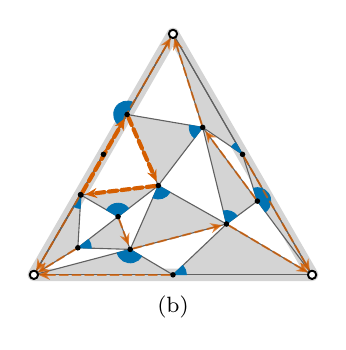
\begin{tikzpicture}[bf,x=0.03364\textwidth,y=0.03364\textwidth]
\draw[bfblack,line width=4.5pt,line join=round] (-4.330,-2.500)--(4.330,-2.500)--(0.000,5.000)--cycle;
\fill[bfblack] (-4.330,-2.500)--(-2.165,1.250)--(-2.879,-0.004)--cycle;
\fill[bfblack] (-4.330,-2.500)--(-2.866,-0.015)--(-2.962,-1.658)--cycle;
\fill[bfblack] (-4.330,-2.500)--(-1.333,-1.708)--(-0.000,-2.500)--cycle;
\fill[bfblack] (4.330,-2.500)--(-0.000,-2.500)--(1.665,-0.918)--cycle;
\fill[bfblack] (4.330,-2.500)--(2.627,-0.205)--(2.165,1.250)--cycle;
\fill[bfblack] (0.000,5.000)--(-2.165,1.250)--(-1.428,2.491)--cycle;
\fill[bfblack] (0.000,5.000)--(2.165,1.250)--(0.925,2.090)--cycle;
\fill[bfblack] (-2.879,-0.004)--(-2.866,-0.015)--(-1.428,2.491)--cycle;
\fill[bfblack] (-2.866,-0.015)--(-0.457,0.279)--(-1.710,-0.689)--cycle;
\fill[bfblack] (-2.962,-1.658)--(-1.333,-1.708)--(-1.710,-0.689)--cycle;
\fill[bfblack] (-1.333,-1.708)--(1.665,-0.918)--(-0.457,0.279)--cycle;
\fill[bfblack] (1.665,-0.918)--(2.627,-0.205)--(0.925,2.090)--cycle;
\fill[bfblack] (0.925,2.090)--(-1.428,2.491)--(-0.457,0.279)--cycle;
\draw[bf edge] (-4.330,-2.500)--(4.330,-2.500);
\draw[bf edge] (-4.330,-2.500)--(0.000,5.000);
\draw[bf edge] (-4.330,-2.500)--(-2.165,1.250);
\draw[bf edge] (-4.330,-2.500)--(-2.879,-0.004);
\draw[bf edge] (-4.330,-2.500)--(-2.866,-0.015);
\draw[bf edge] (-4.330,-2.500)--(-2.962,-1.658);
\draw[bf edge] (-4.330,-2.500)--(-1.333,-1.708);
\draw[bf edge] (-4.330,-2.500)--(-0.000,-2.500);
\draw[bf edge] (4.330,-2.500)--(0.000,5.000);
\draw[bf edge] (4.330,-2.500)--(-0.000,-2.500);
\draw[bf edge] (4.330,-2.500)--(1.665,-0.918);
\draw[bf edge] (4.330,-2.500)--(2.627,-0.205);
\draw[bf edge] (4.330,-2.500)--(2.165,1.250);
\draw[bf edge] (0.000,5.000)--(-2.165,1.250);
\draw[bf edge] (0.000,5.000)--(2.165,1.250);
\draw[bf edge] (0.000,5.000)--(0.925,2.090);
\draw[bf edge] (0.000,5.000)--(-1.428,2.491);
\draw[bf edge] (-2.165,1.250)--(-2.879,-0.004);
\draw[bf edge] (-2.165,1.250)--(-1.428,2.491);
\draw[bf edge] (-2.879,-0.004)--(-2.866,-0.015);
\draw[bf edge] (-2.879,-0.004)--(-1.428,2.491);
\draw[bf edge] (-2.866,-0.015)--(-2.962,-1.658);
\draw[bf edge] (-2.866,-0.015)--(-1.428,2.491);
\draw[bf edge] (-2.866,-0.015)--(-0.457,0.279);
\draw[bf edge] (-2.866,-0.015)--(-1.710,-0.689);
\draw[bf edge] (-2.962,-1.658)--(-1.333,-1.708);
\draw[bf edge] (-2.962,-1.658)--(-1.710,-0.689);
\draw[bf edge] (-1.333,-1.708)--(-0.000,-2.500);
\draw[bf edge] (-1.333,-1.708)--(1.665,-0.918);
\draw[bf edge] (-1.333,-1.708)--(-0.457,0.279);
\draw[bf edge] (-1.333,-1.708)--(-1.710,-0.689);
\draw[bf edge] (-0.000,-2.500)--(1.665,-0.918);
\draw[bf edge] (1.665,-0.918)--(2.627,-0.205);
\draw[bf edge] (1.665,-0.918)--(0.925,2.090);
\draw[bf edge] (1.665,-0.918)--(-0.457,0.279);
\draw[bf edge] (2.627,-0.205)--(2.165,1.250);
\draw[bf edge] (2.627,-0.205)--(0.925,2.090);
\draw[bf edge] (2.165,1.250)--(0.925,2.090);
\draw[bf edge] (0.925,2.090)--(-1.428,2.491);
\draw[bf edge] (0.925,2.090)--(-0.457,0.279);
\draw[bf edge] (-1.428,2.491)--(-0.457,0.279);
\draw[bf edge] (-0.457,0.279)--(-1.710,-0.689);
\path[bf s] (-2.165,1.250) -- ++(-120.0:0.420) arc[start angle=-120.0,end angle=-119.7,radius=0.420] -- cycle;
\path[bf s] (-2.866,-0.015) -- ++(-120.5:0.420) arc[start angle=-120.5,end angle=-93.3,radius=0.420] -- cycle;
\path[bf s] (-1.333,-1.708) -- ++(-165.2:0.420) arc[start angle=-165.2,end angle=-30.7,radius=0.420] -- cycle;
\path[bf s] (-0.000,-2.500) -- ++(-0.0:0.420) arc[start angle=-0.0,end angle=43.5,radius=0.420] -- cycle;
\path[bf s] (2.627,-0.205) -- ++(-53.4:0.420) arc[start angle=-53.4,end angle=107.6,radius=0.420] -- cycle;
\path[bf s] (-1.428,2.491) -- ++(60.3:0.420) arc[start angle=60.3,end angle=239.3,radius=0.420] -- cycle;
\path[bf s] (2.165,1.250) -- ++(120.0:0.420) arc[start angle=120.0,end angle=145.9,radius=0.420] -- cycle;
\path[bf s] (-2.879,-0.004) -- ++(-39.0:0.007) arc[start angle=-39.0,end angle=59.8,radius=0.007] -- cycle;
\path[bf s] (-1.710,-0.689) -- ++(149.8:0.420) arc[start angle=149.8,end angle=37.7,radius=0.420] -- cycle;
\path[bf s] (-2.962,-1.658) -- ++(-1.8:0.420) arc[start angle=-1.8,end angle=37.8,radius=0.420] -- cycle;
\path[bf s] (-0.457,0.279) -- ++(-113.8:0.420) arc[start angle=-113.8,end angle=-29.4,radius=0.420] -- cycle;
\path[bf s] (1.665,-0.918) -- ++(36.5:0.420) arc[start angle=36.5,end angle=103.8,radius=0.420] -- cycle;
\path[bf s] (0.925,2.090) -- ++(170.3:0.420) arc[start angle=170.3,end angle=232.7,radius=0.420] -- cycle;
\draw[bf Qdir,line width=.7pt,opacity=.75] (-2.879,-0.004) to[bend left=0] (-4.330,-2.500);
\draw[bf Qdir,line width=.7pt,opacity=.75] (-2.962,-1.658) to[bend left=0] (-4.330,-2.500);
\draw[bf Qdir,line width=.7pt,opacity=.75] (-0.000,-2.500) to[bend left=0] (-4.330,-2.500);
\draw[bf Qdir,line width=.7pt,opacity=.75] (1.665,-0.918) to[bend left=0] (4.330,-2.500);
\draw[bf Qdir,line width=.7pt,opacity=.75] (2.165,1.250) to[bend left=0] (4.330,-2.500);
\draw[bf Qdir,line width=.7pt,opacity=.75] (-2.165,1.250) to[bend left=0] (0.000,5.000);
\draw[bf Qdir,line width=.7pt,opacity=.75] (0.925,2.090) to[bend left=0] (0.000,5.000);
\draw[bf Qdir,line width=1.5pt] (-2.866,-0.015) to[bend left=0] (-1.428,2.491);
\draw[bf Qdir,line width=1.5pt] (-0.457,0.279) to[bend left=0] (-2.866,-0.015);
\draw[bf Qdir,line width=.7pt,opacity=.75] (-1.710,-0.689) to[bend left=0] (-1.333,-1.708);
\draw[bf Qdir,line width=.7pt,opacity=.75] (-1.333,-1.708) to[bend left=0] (1.665,-0.918);
\draw[bf Qdir,line width=.7pt,opacity=.75] (2.627,-0.205) to[bend left=0] (0.925,2.090);
\draw[bf Qdir,line width=1.5pt] (-1.428,2.491) to[bend left=0] (-0.457,0.279);
\path[bf root] (-4.330,-2.500) circle[radius=1.5pt];
\path[bf root] (4.330,-2.500) circle[radius=1.5pt];
\path[bf root] (0.000,5.000) circle[radius=1.5pt];
\path[bf vertex] (-2.165,1.250) circle[radius=1.0pt];
\path[bf vertex] (-2.879,-0.004) circle[radius=1.0pt];
\path[bf vertex] (-2.866,-0.015) circle[radius=1.0pt];
\path[bf vertex] (-2.962,-1.658) circle[radius=1.0pt];
\path[bf vertex] (-1.333,-1.708) circle[radius=1.0pt];
\path[bf vertex] (-0.000,-2.500) circle[radius=1.0pt];
\path[bf vertex] (1.665,-0.918) circle[radius=1.0pt];
\path[bf vertex] (2.627,-0.205) circle[radius=1.0pt];
\path[bf vertex] (2.165,1.250) circle[radius=1.0pt];
\path[bf vertex] (0.925,2.090) circle[radius=1.0pt];
\path[bf vertex] (-1.428,2.491) circle[radius=1.0pt];
\path[bf vertex] (-0.457,0.279) circle[radius=1.0pt];
\path[bf vertex] (-1.710,-0.689) circle[radius=1.0pt];
\node[anchor=north] at (0.000,-3.050) {(b)};
\end{tikzpicture}%
\hfill%
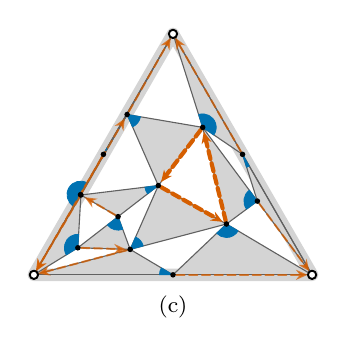
\begin{tikzpicture}[bf,x=0.03364\textwidth,y=0.03364\textwidth]
\draw[bfblack,line width=4.5pt,line join=round] (-4.330,-2.500)--(4.330,-2.500)--(0.000,5.000)--cycle;
\fill[bfblack] (-4.330,-2.500)--(-2.165,1.250)--(-2.879,-0.004)--cycle;
\fill[bfblack] (-4.330,-2.500)--(-2.866,-0.015)--(-2.962,-1.658)--cycle;
\fill[bfblack] (-4.330,-2.500)--(-1.333,-1.708)--(-0.000,-2.500)--cycle;
\fill[bfblack] (4.330,-2.500)--(-0.000,-2.500)--(1.665,-0.918)--cycle;
\fill[bfblack] (4.330,-2.500)--(2.627,-0.205)--(2.165,1.250)--cycle;
\fill[bfblack] (0.000,5.000)--(-2.165,1.250)--(-1.428,2.491)--cycle;
\fill[bfblack] (0.000,5.000)--(2.165,1.250)--(0.925,2.090)--cycle;
\fill[bfblack] (-2.879,-0.004)--(-2.866,-0.015)--(-1.428,2.491)--cycle;
\fill[bfblack] (-2.866,-0.015)--(-0.457,0.279)--(-1.710,-0.689)--cycle;
\fill[bfblack] (-2.962,-1.658)--(-1.333,-1.708)--(-1.710,-0.689)--cycle;
\fill[bfblack] (-1.333,-1.708)--(1.665,-0.918)--(-0.457,0.279)--cycle;
\fill[bfblack] (1.665,-0.918)--(2.627,-0.205)--(0.925,2.090)--cycle;
\fill[bfblack] (0.925,2.090)--(-1.428,2.491)--(-0.457,0.279)--cycle;
\draw[bf edge] (-4.330,-2.500)--(4.330,-2.500);
\draw[bf edge] (-4.330,-2.500)--(0.000,5.000);
\draw[bf edge] (-4.330,-2.500)--(-2.165,1.250);
\draw[bf edge] (-4.330,-2.500)--(-2.879,-0.004);
\draw[bf edge] (-4.330,-2.500)--(-2.866,-0.015);
\draw[bf edge] (-4.330,-2.500)--(-2.962,-1.658);
\draw[bf edge] (-4.330,-2.500)--(-1.333,-1.708);
\draw[bf edge] (-4.330,-2.500)--(-0.000,-2.500);
\draw[bf edge] (4.330,-2.500)--(0.000,5.000);
\draw[bf edge] (4.330,-2.500)--(-0.000,-2.500);
\draw[bf edge] (4.330,-2.500)--(1.665,-0.918);
\draw[bf edge] (4.330,-2.500)--(2.627,-0.205);
\draw[bf edge] (4.330,-2.500)--(2.165,1.250);
\draw[bf edge] (0.000,5.000)--(-2.165,1.250);
\draw[bf edge] (0.000,5.000)--(2.165,1.250);
\draw[bf edge] (0.000,5.000)--(0.925,2.090);
\draw[bf edge] (0.000,5.000)--(-1.428,2.491);
\draw[bf edge] (-2.165,1.250)--(-2.879,-0.004);
\draw[bf edge] (-2.165,1.250)--(-1.428,2.491);
\draw[bf edge] (-2.879,-0.004)--(-2.866,-0.015);
\draw[bf edge] (-2.879,-0.004)--(-1.428,2.491);
\draw[bf edge] (-2.866,-0.015)--(-2.962,-1.658);
\draw[bf edge] (-2.866,-0.015)--(-1.428,2.491);
\draw[bf edge] (-2.866,-0.015)--(-0.457,0.279);
\draw[bf edge] (-2.866,-0.015)--(-1.710,-0.689);
\draw[bf edge] (-2.962,-1.658)--(-1.333,-1.708);
\draw[bf edge] (-2.962,-1.658)--(-1.710,-0.689);
\draw[bf edge] (-1.333,-1.708)--(-0.000,-2.500);
\draw[bf edge] (-1.333,-1.708)--(1.665,-0.918);
\draw[bf edge] (-1.333,-1.708)--(-0.457,0.279);
\draw[bf edge] (-1.333,-1.708)--(-1.710,-0.689);
\draw[bf edge] (-0.000,-2.500)--(1.665,-0.918);
\draw[bf edge] (1.665,-0.918)--(2.627,-0.205);
\draw[bf edge] (1.665,-0.918)--(0.925,2.090);
\draw[bf edge] (1.665,-0.918)--(-0.457,0.279);
\draw[bf edge] (2.627,-0.205)--(2.165,1.250);
\draw[bf edge] (2.627,-0.205)--(0.925,2.090);
\draw[bf edge] (2.165,1.250)--(0.925,2.090);
\draw[bf edge] (0.925,2.090)--(-1.428,2.491);
\draw[bf edge] (0.925,2.090)--(-0.457,0.279);
\draw[bf edge] (-1.428,2.491)--(-0.457,0.279);
\draw[bf edge] (-0.457,0.279)--(-1.710,-0.689);
\path[bf s] (-2.879,-0.004) -- ++(-120.2:0.420) arc[start angle=-120.2,end angle=-299.7,radius=0.420] -- cycle;
\path[bf s] (-2.962,-1.658) -- ++(-148.4:0.420) arc[start angle=-148.4,end angle=-273.3,radius=0.420] -- cycle;
\path[bf s] (-0.000,-2.500) -- ++(-180.0:0.420) arc[start angle=-180.0,end angle=-210.7,radius=0.420] -- cycle;
\path[bf s] (1.665,-0.918) -- ++(-30.7:0.420) arc[start angle=-30.7,end angle=-136.5,radius=0.420] -- cycle;
\path[bf s] (2.165,1.250) -- ++(-60.0:0.420) arc[start angle=-60.0,end angle=-72.4,radius=0.420] -- cycle;
\path[bf s] (-2.165,1.250) -- ++(60.0:0.420) arc[start angle=60.0,end angle=59.3,radius=0.420] -- cycle;
\path[bf s] (0.925,2.090) -- ++(107.6:0.420) arc[start angle=107.6,end angle=-34.1,radius=0.420] -- cycle;
\path[bf s] (-2.866,-0.015) -- ++(141.0:0.007) arc[start angle=141.0,end angle=60.2,radius=0.007] -- cycle;
\path[bf s] (-0.457,0.279) -- ++(-173.1:0.420) arc[start angle=-173.1,end angle=-142.3,radius=0.420] -- cycle;
\path[bf s] (-1.710,-0.689) -- ++(-142.2:0.420) arc[start angle=-142.2,end angle=-69.7,radius=0.420] -- cycle;
\path[bf s] (-1.333,-1.708) -- ++(14.8:0.420) arc[start angle=14.8,end angle=66.2,radius=0.420] -- cycle;
\path[bf s] (2.627,-0.205) -- ++(-143.5:0.420) arc[start angle=-143.5,end angle=-233.4,radius=0.420] -- cycle;
\path[bf s] (-1.428,2.491) -- ++(-9.7:0.420) arc[start angle=-9.7,end angle=-66.3,radius=0.420] -- cycle;
\draw[bf Qdir,line width=.7pt,opacity=.75] (-2.165,1.250) to[bend left=0] (-4.330,-2.500);
\draw[bf Qdir,line width=.7pt,opacity=.75] (-2.866,-0.015) to[bend left=0] (-4.330,-2.500);
\draw[bf Qdir,line width=.7pt,opacity=.75] (-1.333,-1.708) to[bend left=0] (-4.330,-2.500);
\draw[bf Qdir,line width=.7pt,opacity=.75] (-0.000,-2.500) to[bend left=0] (4.330,-2.500);
\draw[bf Qdir,line width=.7pt,opacity=.75] (2.627,-0.205) to[bend left=0] (4.330,-2.500);
\draw[bf Qdir,line width=.7pt,opacity=.75] (-1.428,2.491) to[bend left=0] (0.000,5.000);
\draw[bf Qdir,line width=.7pt,opacity=.75] (2.165,1.250) to[bend left=0] (0.000,5.000);
\draw[bf Qdir,line width=.7pt,opacity=.75] (-2.879,-0.004) to[bend left=0] (-1.428,2.491);
\draw[bf Qdir,line width=.7pt,opacity=.75] (-1.710,-0.689) to[bend left=0] (-2.866,-0.015);
\draw[bf Qdir,line width=.7pt,opacity=.75] (-2.962,-1.658) to[bend left=0] (-1.333,-1.708);
\draw[bf Qdir,line width=1.5pt] (-0.457,0.279) to[bend left=0] (1.665,-0.918);
\draw[bf Qdir,line width=1.5pt] (1.665,-0.918) to[bend left=0] (0.925,2.090);
\draw[bf Qdir,line width=1.5pt] (0.925,2.090) to[bend left=0] (-0.457,0.279);
\path[bf root] (-4.330,-2.500) circle[radius=1.5pt];
\path[bf root] (4.330,-2.500) circle[radius=1.5pt];
\path[bf root] (0.000,5.000) circle[radius=1.5pt];
\path[bf vertex] (-2.165,1.250) circle[radius=1.0pt];
\path[bf vertex] (-2.879,-0.004) circle[radius=1.0pt];
\path[bf vertex] (-2.866,-0.015) circle[radius=1.0pt];
\path[bf vertex] (-2.962,-1.658) circle[radius=1.0pt];
\path[bf vertex] (-1.333,-1.708) circle[radius=1.0pt];
\path[bf vertex] (-0.000,-2.500) circle[radius=1.0pt];
\path[bf vertex] (1.665,-0.918) circle[radius=1.0pt];
\path[bf vertex] (2.627,-0.205) circle[radius=1.0pt];
\path[bf vertex] (2.165,1.250) circle[radius=1.0pt];
\path[bf vertex] (0.925,2.090) circle[radius=1.0pt];
\path[bf vertex] (-1.428,2.491) circle[radius=1.0pt];
\path[bf vertex] (-0.457,0.279) circle[radius=1.0pt];
\path[bf vertex] (-1.710,-0.689) circle[radius=1.0pt];
\node[anchor=north] at (0.000,-3.050) {(c)};
\end{tikzpicture}%
\end{minipage}}
\caption{The $2$-factor $F$ of Proposition~\ref{prop:bad}. (a) The triangulation, with the grey ring standing for $t_0=\{0,1,2\}$, and for every $t\in A$ the side of $t$ opposite $u(t)$; these sides form the cycle of $D(r,s)$ for the two pairs $(r,s)$ with $2$-factor $F$, through the $13$ vertices of $X$. (b) One of the two states $s$ in $F$, marked by wedges, with $Q_s$ directed from $r(t)$ to $u(t)$ in dashed arrows; the directed triangle $5\to13\to14\to5$ is bold. (c) The other state; the directed triangle is $9\to12\to14\to9$.}
\label{fig:bad}
\end{figure}

By enumeration, every $2$-factor contains a good state when $T$ has at most $12$ vertices and a pair.
Theorems~\ref{thm:twotrees} to~\ref{thm:edmonds} hold for every $2$-factor, the one of Proposition~\ref{prop:bad} included, and so cannot tell a $2$-factor that contains a good state from one that does not.
Hence no argument that stays in one $2$-factor can prove \cite[Proposition~6.9]{Paper}.
The signed proof does not stay in one $2$-factor either: the cancellation of \cite[Lemma~5.6]{Paper} replaces $r$ by $r^K$ for a cycle $K$ of $Q_s$, which changes the $2$-factor, and the evaluation in \cite[Proposition~6.9]{Paper} sums over all $2$-factors with $m$ cycles.

\subsection*{The missing step}

\begin{conjecture}\label{conj:X}
Suppose that no separating triangle of $T$ has three black faces along its inner side.
Then for every rainbow tree $\sigma$ there are rainbow trees $\sigma=\sigma_0,\sigma_1,\dots,\sigma_k$ such that $\sigma_{i+1}$ arises from $\sigma_i$ by one exchange, $\exc(\sigma_{i+1})\le\exc(\sigma_i)$ for all $i$, and $\exc(\sigma_k)=0$.
\end{conjecture}

With Theorem~\ref{thm:R} and Lemma~\ref{lem:good} this implies \cite[Proposition~6.9]{Paper}.
By enumeration, the conjecture holds for every choice of $t_0$ in every Eulerian triangulation with at most $17$ vertices.
It also holds when $H$ has only one $2$-factor $F$.
Then all maps that lie in $F$ are rainbow trees by Theorem~\ref{thm:S}(3), and one can move a vertex of a face of load $2$ to its other face in $F$, then the vertex that was already in that face onwards in the same direction along the cycle of $F$, and so on; this reaches a face of load $0$ without raising the excess.

Three stronger statements would give a proof or an algorithm at once, and all three fail.

\emph{Strict descent.}
A rainbow tree of positive excess need not have an exchange that lowers the excess; the smallest examples are in the triangulation with $8$ vertices.
So a sequence as in Conjecture~\ref{conj:X} must pass through rainbow trees of equal excess.

\emph{The walk.}
The walk of Section~\ref{sec:even}, started at an arbitrary walk state, need not stop.
There are periodic walks in triangulations with $38$ and with $40$ vertices; by enumeration there is none up to $15$ vertices.
The walks of Theorem~\ref{thm:even} stop only because their first walk state is not in the image of $\step$.

\emph{Convexity of loads.}
If the set of the load vectors $(\lambda_\sigma(t))_{t\in A}$ of the rainbow trees satisfied the exchange axiom of M-convex sets, a condition of Hall's type would decide whether the vector with all loads $1$ belongs to it.
The axiom fails in a triangulation with $12$ vertices in which $H$ has two $2$-factors.

The involutions $\iota_t$ do not connect the good states either: there are triangulations with $13$ and with $14$ vertices in which the group they generate is not transitive on the good states.

A statement of the same kind can be made for pairs, with the two modifications of \cite[Sections~5 and~6]{Paper}: replacing $r$ by $r^K$ for a cycle $K$ of $Q_s$, and reversing a cycle of $D(r,s)$.
By enumeration up to $20$ vertices, every pair can be turned by such modifications into a pair with a good second state without ever raising the number of cycles of $Q_s$.
A modification that lowers this number need not exist, first for $16$ vertices, and for $16$ vertices it is not always possible to proceed without raising $c(F)$.
So here too the number that should reach zero cannot be lowered step by step, the modifications that keep it constant change the $2$-factor, and we know no quantity that decreases along them.
The exchange procedure of \cite{Constructive} mentioned in the Remarks of \cite{Paper} does reach a good state, but it follows the signed cancellation.

\subsection*{What a proof of the conjecture would give}
Suppose that Conjecture~\ref{conj:X} were proved.
Theorem~\ref{thm:R} supplies a rainbow tree whenever no separating triangle has three black faces along its inner side, and the conjecture leads from it to a good state.
That is \cite[Proposition~6.9]{Paper} with no sign, no weight and no sum over $2$-factors, and Theorem~\ref{thm:even} then gives a second good state.
The rest of the proof in \cite{Paper} uses no cancellation: \cite[Proposition~3.5]{Paper} leads from a good state to a Hamiltonian cycle, and the induction in \cite[Proposition~2.7]{Paper} deals with the separating triangles.
A proof of the conjecture would not give a polynomial algorithm, since the conjecture only asserts that a sequence of exchanges exists and nothing bounds the search among rainbow trees of equal excess.
Nor would it count the good states or explain why the signed sum does not vanish.

The place to look is the exchange that leaves the $2$-factor, which Section~\ref{sec:packing} does not see.
A rainbow tree in $F$ is an acyclic choice of arcs in $D_F$, its excess is the number of faces with both arcs or no arc chosen, and correcting a face along a cycle of $F$ works until the new arc closes a directed cycle.
In the signed proof this is a cycle of $Q_s$, and the disk identity \cite[Lemma~5.1]{Paper} controls it there.
The disk identity is not used in this note, and we expect that a proof of Conjecture~\ref{conj:X} has to use it.

\begin{thebibliography}{9}
\bibitem{Constructive} \emph{A constructive proof of Barnette's conjecture}, anonymous unpublished manuscript, 18 October 2026.
\bibitem{Diestel} R.~Diestel, \emph{Graph theory}, 5th ed., Graduate Texts in Mathematics, vol.~173, Springer, Berlin, 2017.
\bibitem{Edmonds} J.~Edmonds, \emph{Edge-disjoint branchings}, Combinatorial Algorithms (R.~Rustin, ed.), Academic Press, New York, 1973, pp.~91--96.
\bibitem{Li} Z.~Li, \emph{A note on the proof of Barnette's conjecture}, preprint, arXiv:2610.30490, 2026.
\bibitem{NashWilliams} C.~St.\,J.~A. Nash-Williams, \emph{Decomposition of finite graphs into forests}, J. London Math. Soc. \textbf{39} (1964), 12.
\bibitem{OpenAI} OpenAI, \emph{Paired states and Hamiltonian cycles in cubic bipartite planar graphs}, preprint, 24 September 2026, \url{https://github.com/openai/math}.
\bibitem{Paper} \emph{The proof of Barnette's conjecture}, exposition, \texttt{paper/barnette.pdf} in this repository.
\bibitem{Rado} R.~Rado, \emph{A theorem on independence relations}, Quart. J. Math. Oxford Ser. \textbf{13} (1942), 83--89.
\bibitem{SchrijverCourse} A.~Schrijver, \emph{A course in combinatorial optimization}, lecture notes, CWI, Amsterdam, 2017.
\bibitem{SchrijverHandbook} A.~Schrijver, \emph{Polyhedral combinatorics}, Handbook of Combinatorics (R.~L. Graham, M.~Gr\"otschel, and L.~Lov\'asz, eds.), Elsevier, Amsterdam, 1995, pp.~1649--1704.
\end{thebibliography}

\end{document}
